\section{Event Selection}
\label{sec:event_selection}

The expected number of signal events in the data is expected
to be very small compared to the total dataset. %give a number
Fortunately, the three lepton signature of the signal allows us to
quickly throw out many events which do not looke like the signal.
Still, this signature is not unique enough that the background
is small. Thus, we must devise a clever way to discriminate 
between the signal and these backgrounds. We select
events in two stages: first we start
by selecting events which have the general signature of the signal, 
this is referred to as the pre-selection stage; then we 
use more stringent cuts to discriminate between the signal and backgrounds, 
referred to as our signal region selection.
The signal region selection is determined starting from the pre-selection
stage by performing an optimization procedure that minimizes the uncertainty
on the final measurement.  This is described in \sec....
The signal region selection is further divided into different
categories that are each used in the final measurement
which allows us to specially treat the different backgrounds
in each category.  
The selections used are described in more detail below.




\subsection{Pre-selection}
\label{sec:preselection}

The pre-selection is determined as a broad selection which throws
away backgrounds that do not at all resemble the signal process.
It is mainly characterized by requiring the presence of exactly three leptons
(electron or muon) following the requirements listed above in 
\sec\ref{sec:object_selection}, each with a $\pt$ of at least $20~\GeV$.
In addition, the events are required to be of good quality. This means
that the events were collected under good conditions during data taking,
both from the LHC operation and ATLAS detector operation. For instance,
during the 2012 data collection, the LAr component of the EM calorimeter
was know to occassionally produce artificial bursts of noise. These instances
were tracked and events where this occured were thrown away. The event is 
also required to have a primary vertex with at least three associted tracks.
Finally, the event is required to pass the single lepton trigger
requirements already listed in \sec\ref{sec:subsection_data} where 
at least one of the three leptons selected caused the trigger to fire.

\begin{figure}[ht!]
\centering
%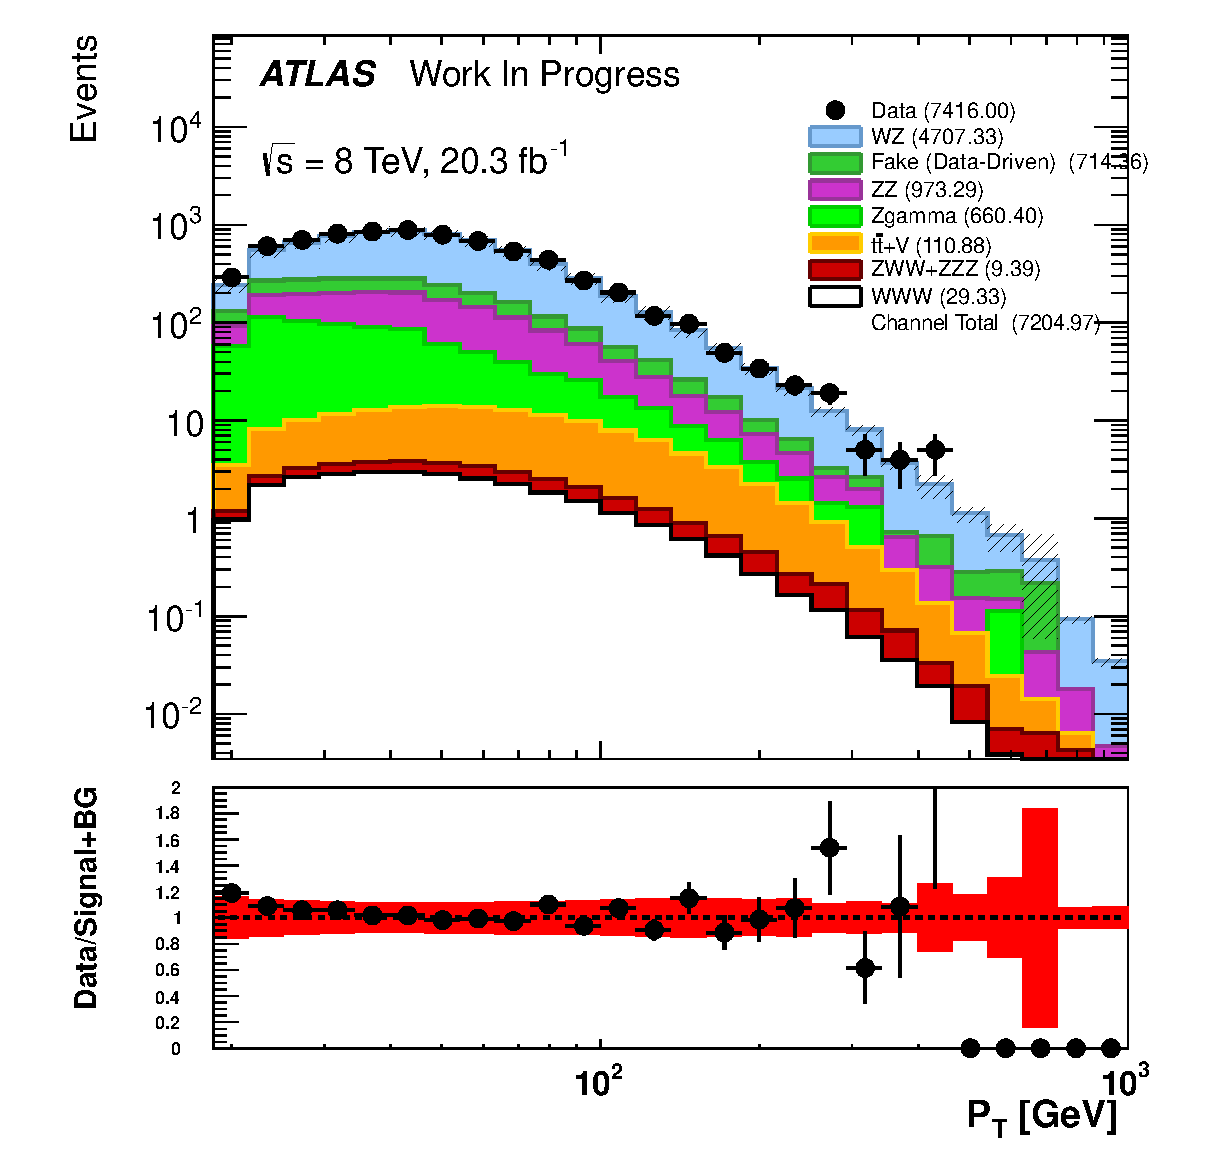
\includegraphics[width=0.3\columnwidth]{figures/appendix_signal_selection/Nov24Update_FakeSys_KFacSys_LogY_NoRebin/output/jobs/MxM/DataFull_Rates_May13_FakeRatesExactly2Loose_MuonMxMBJetGt0_ElBJetGt0SubtractPC_MxM/PreselectionNov23_15_physics/weight_all/eps/AllLeptonPt_histratio.eps}
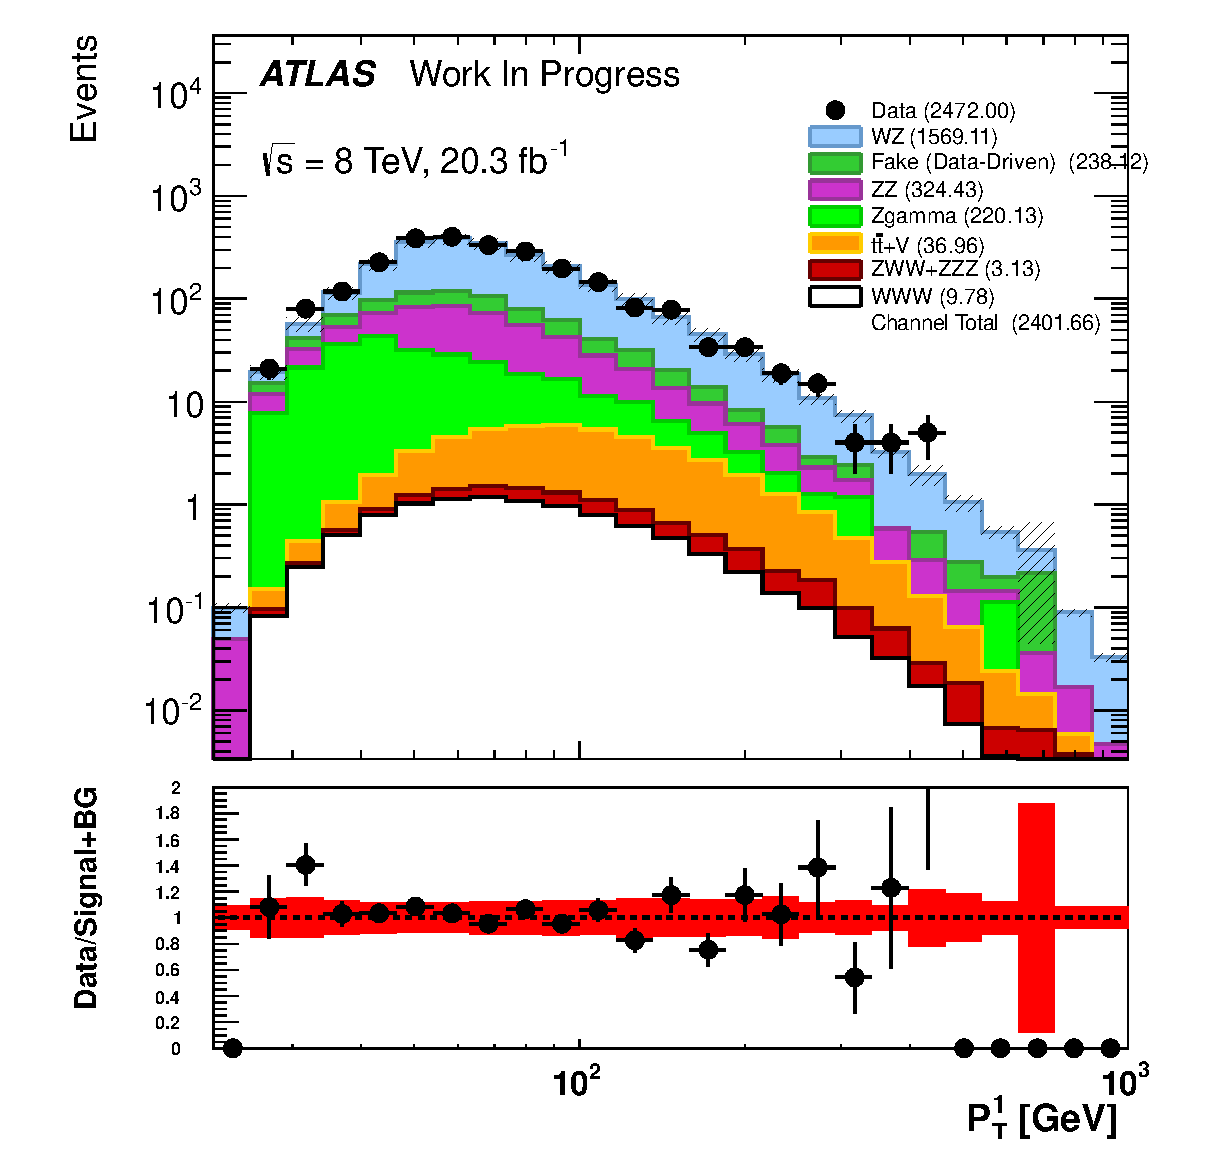
\includegraphics[width=0.3\columnwidth]{figures/appendix_signal_selection/Nov24Update_FakeSys_KFacSys_LogY_NoRebin/output/jobs/MxM/DataFull_Rates_May13_FakeRatesExactly2Loose_MuonMxMBJetGt0_ElBJetGt0SubtractPC_MxM/PreselectionNov23_15_physics/weight_all/eps/LeadingLeptonPt_histratio.eps}
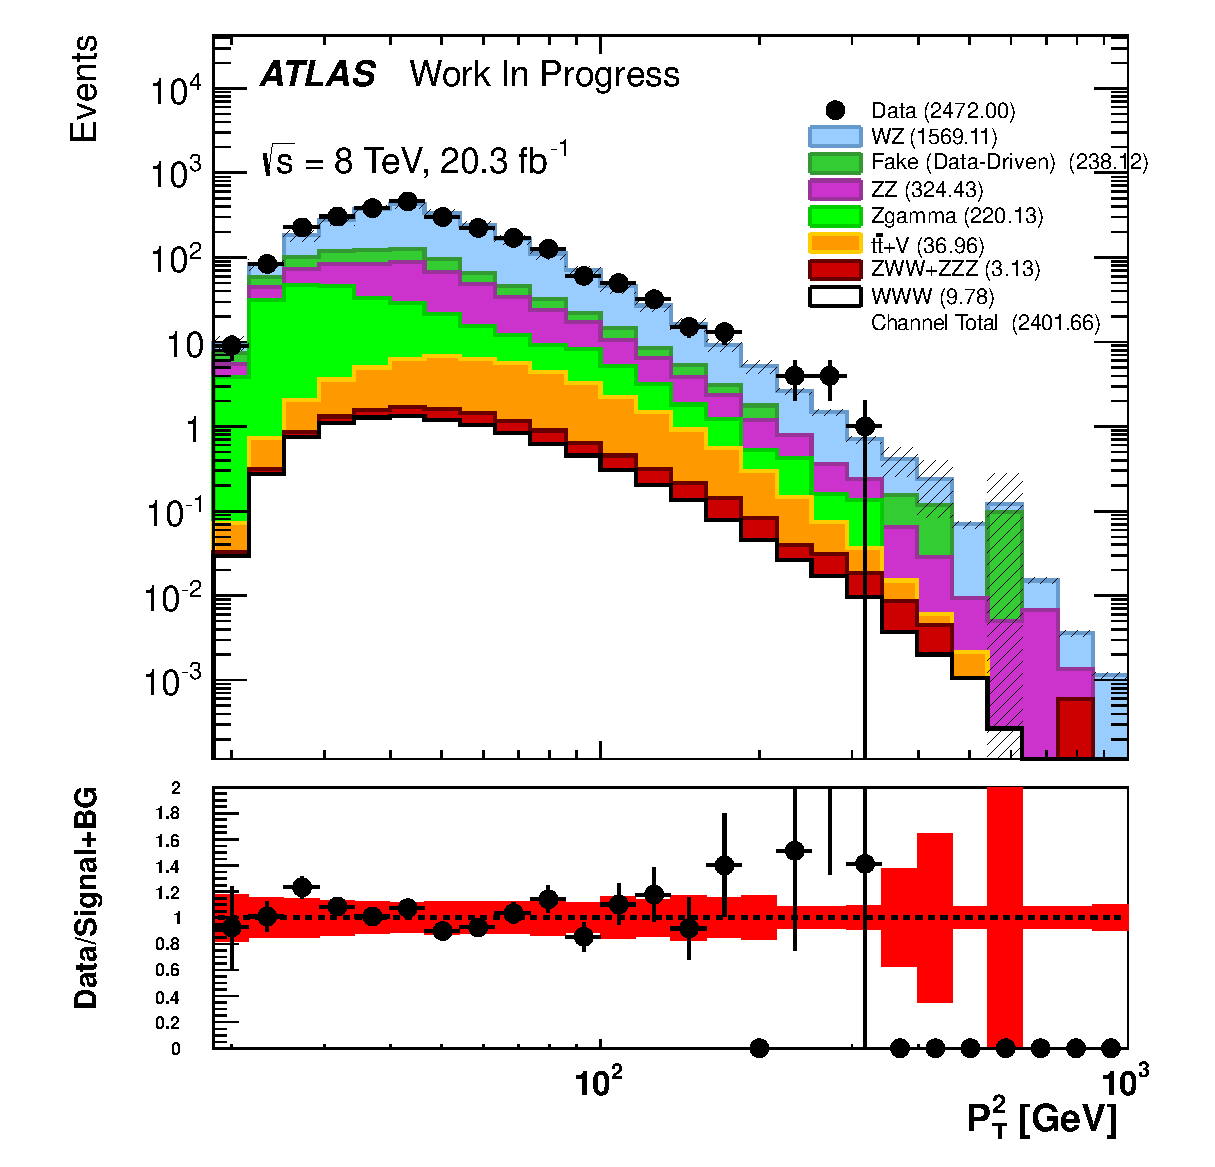
\includegraphics[width=0.3\columnwidth]{figures/appendix_signal_selection/Nov24Update_FakeSys_KFacSys_LogY_NoRebin/output/jobs/MxM/DataFull_Rates_May13_FakeRatesExactly2Loose_MuonMxMBJetGt0_ElBJetGt0SubtractPC_MxM/PreselectionNov23_15_physics/weight_all/eps/SubleadingLeptonPt_histratio.eps}
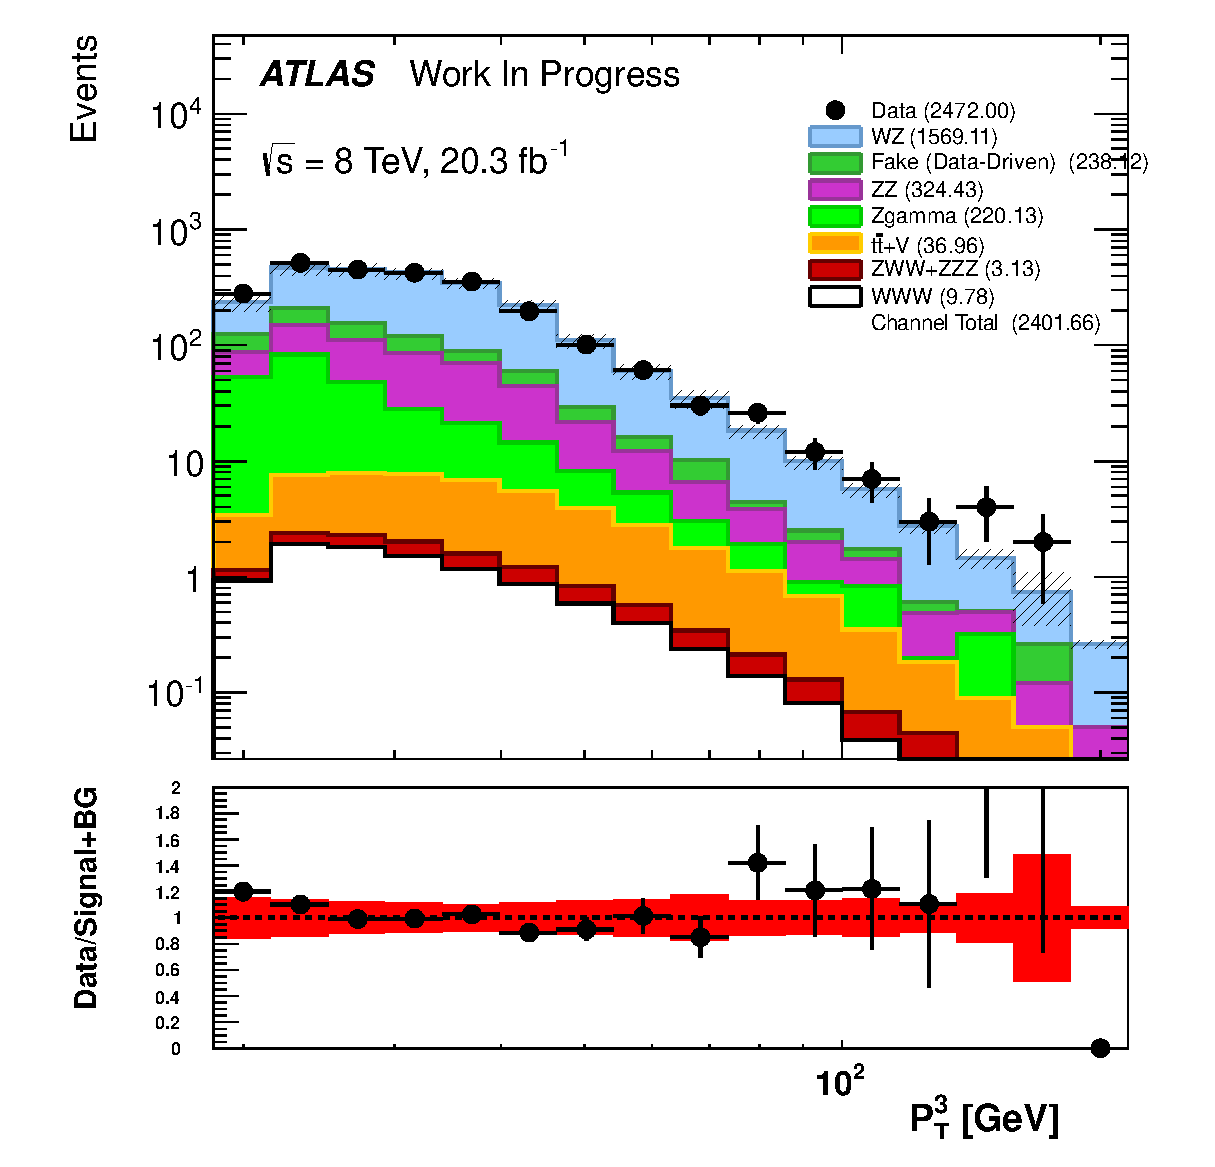
\includegraphics[width=0.3\columnwidth]{figures/appendix_signal_selection/Nov24Update_FakeSys_KFacSys_LogY_NoRebin/output/jobs/MxM/DataFull_Rates_May13_FakeRatesExactly2Loose_MuonMxMBJetGt0_ElBJetGt0SubtractPC_MxM/PreselectionNov23_15_physics/weight_all/eps/MinimumLeptonPt_histratio.eps}
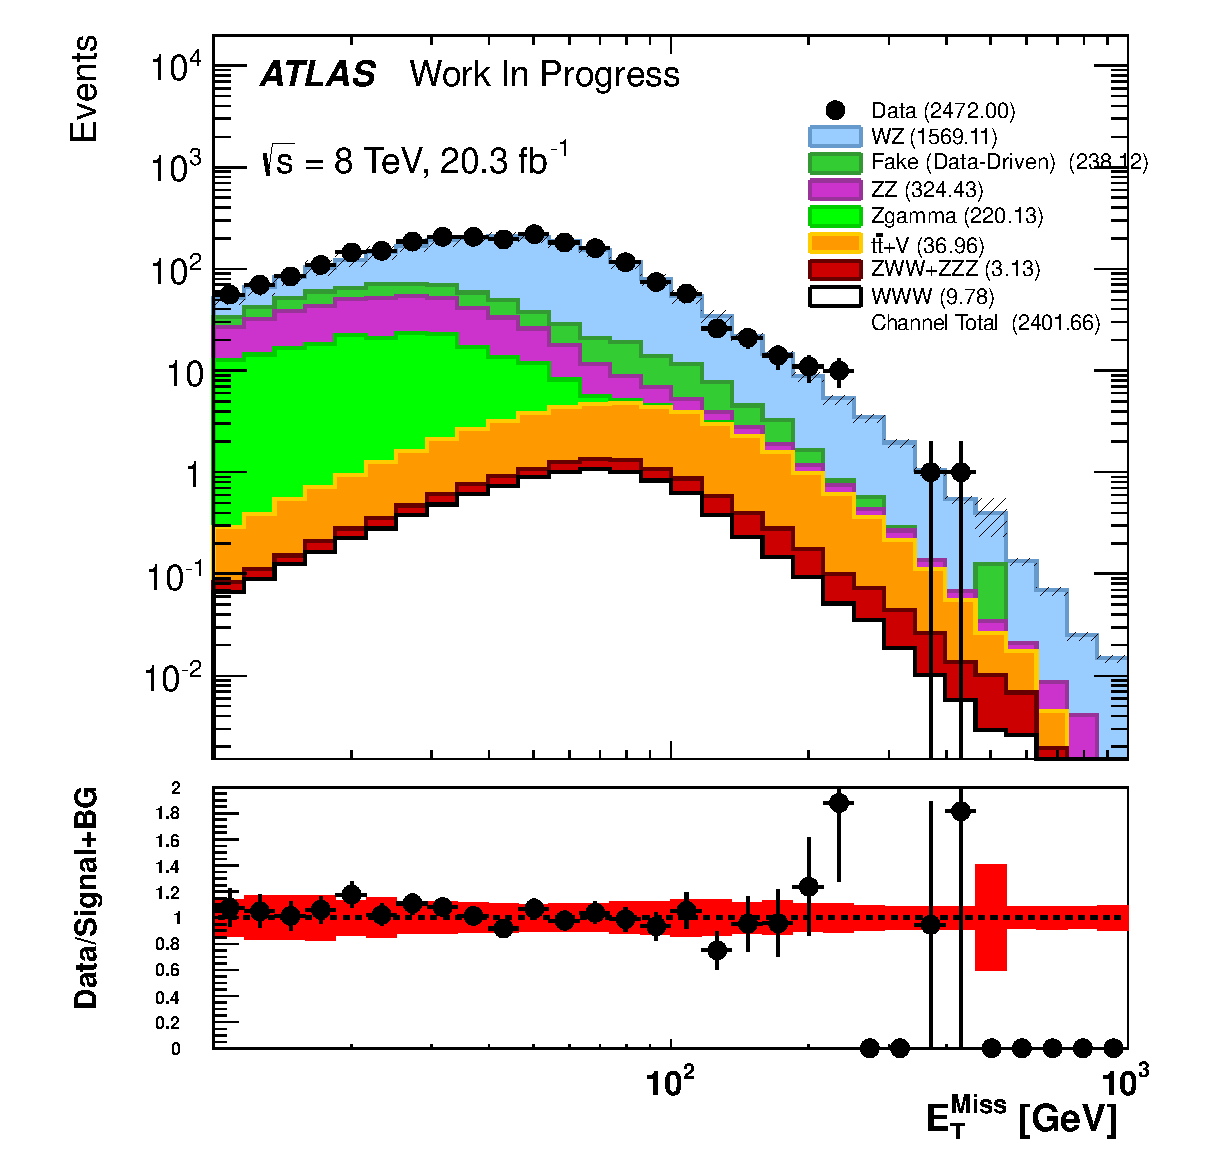
\includegraphics[width=0.3\columnwidth]{figures/appendix_signal_selection/Nov24Update_FakeSys_KFacSys_LogY_NoRebin/output/jobs/MxM/DataFull_Rates_May13_FakeRatesExactly2Loose_MuonMxMBJetGt0_ElBJetGt0SubtractPC_MxM/PreselectionNov23_15_physics/weight_all/eps/MET_Et_histratio.eps}
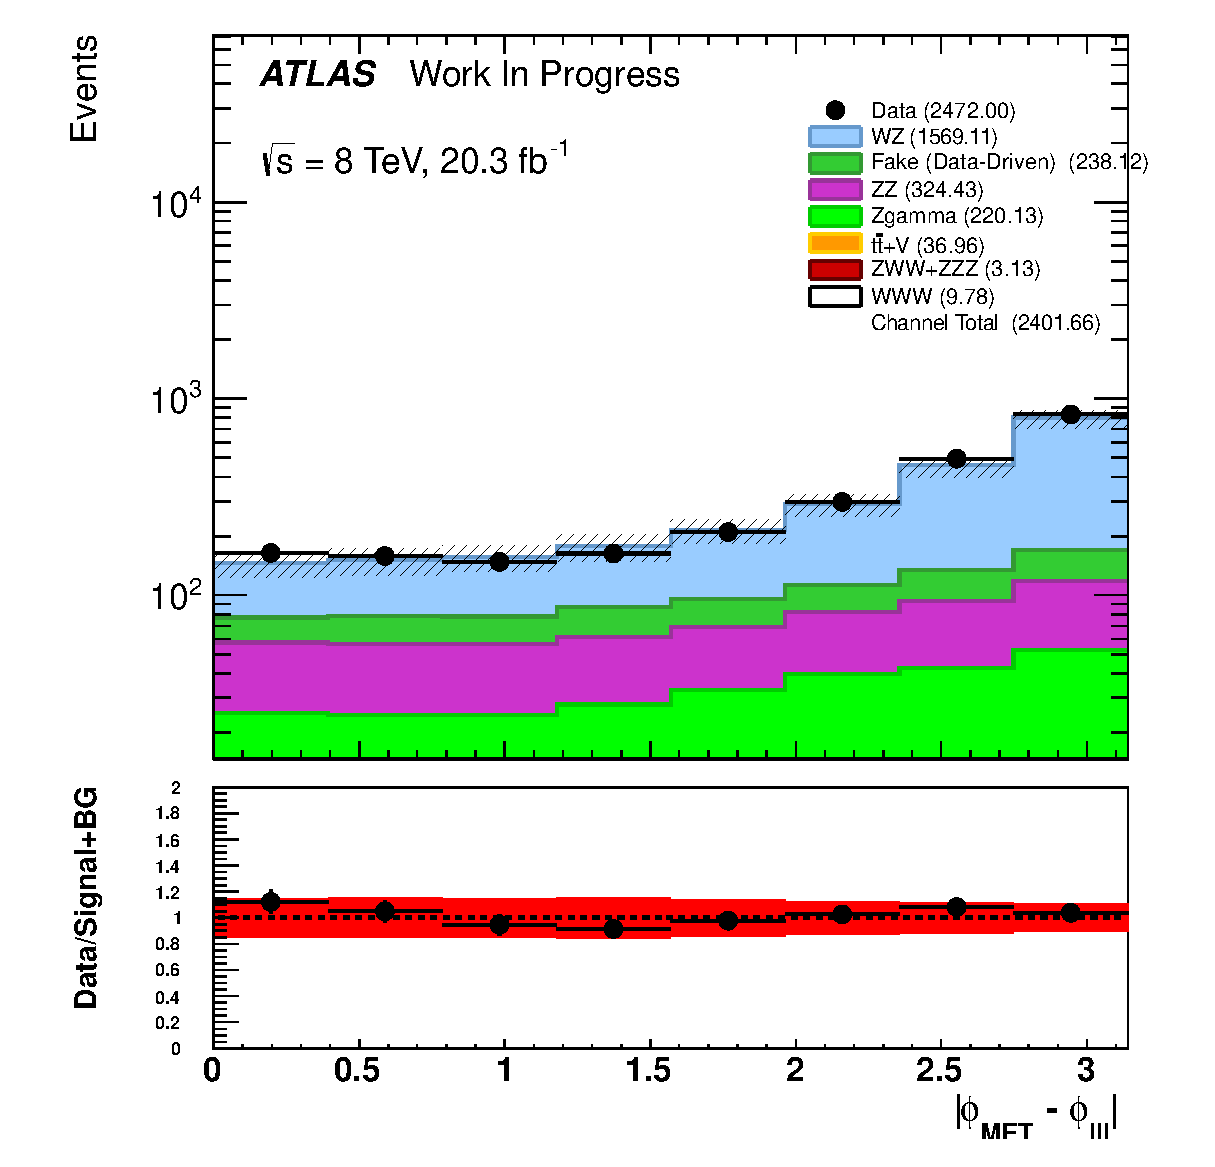
\includegraphics[width=0.3\columnwidth]{figures/appendix_signal_selection/Nov24Update_FakeSys_KFacSys_LogY_NoRebin/output/jobs/MxM/DataFull_Rates_May13_FakeRatesExactly2Loose_MuonMxMBJetGt0_ElBJetGt0SubtractPC_MxM/PreselectionNov23_15_physics/weight_all/eps/DeltaPhiMET123_Abs_histratio.eps}
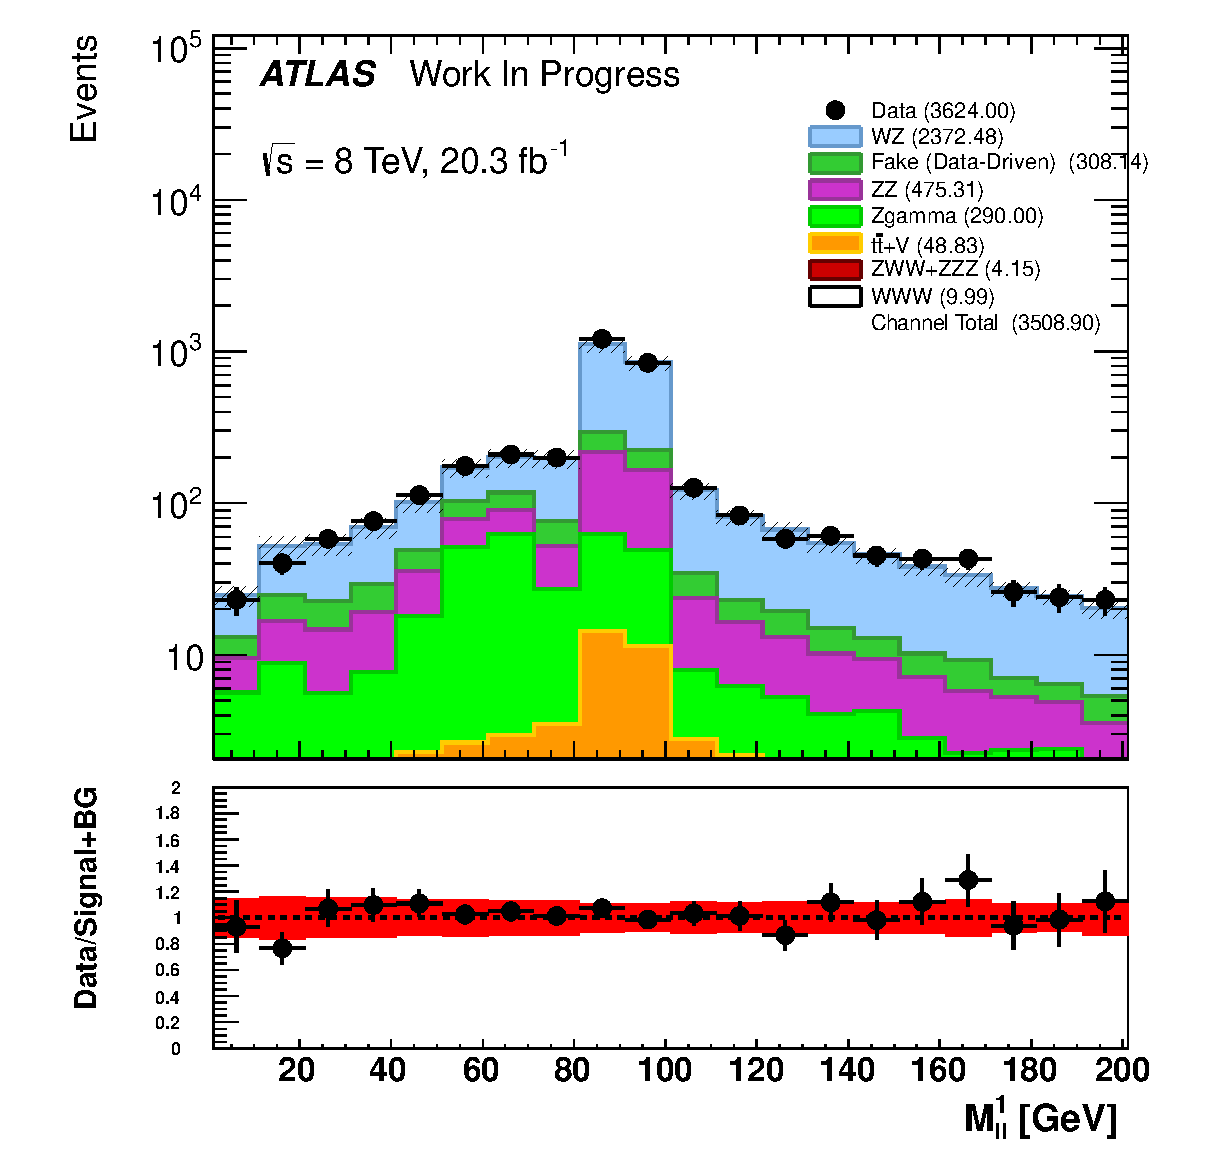
\includegraphics[width=0.3\columnwidth]{figures/appendix_signal_selection/Nov24Update_FakeSys_KFacSys_LogY_NoRebin/output/jobs/MxM/DataFull_Rates_May13_FakeRatesExactly2Loose_MuonMxMBJetGt0_ElBJetGt0SubtractPC_MxM/PreselectionNov23_15_physics/weight_all/eps/InvariantMassSFOS_histratio.eps}
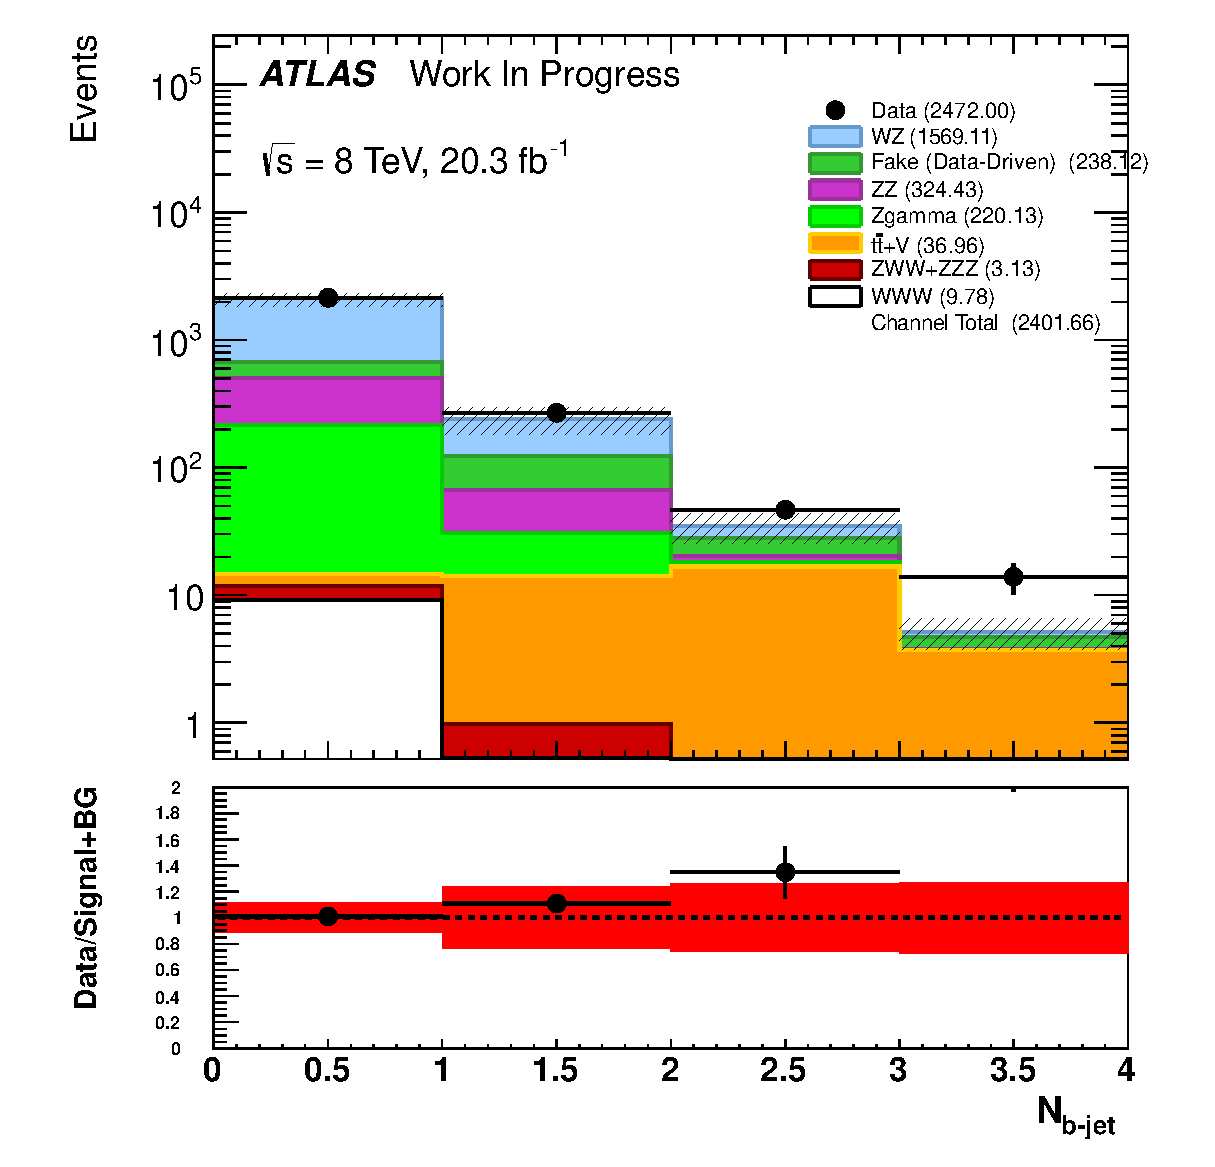
\includegraphics[width=0.3\columnwidth]{figures/appendix_signal_selection/Nov24Update_FakeSys_KFacSys_LogY_NoRebin/output/jobs/MxM/DataFull_Rates_May13_FakeRatesExactly2Loose_MuonMxMBJetGt0_ElBJetGt0SubtractPC_MxM/PreselectionNov23_15_physics/weight_all/eps/NBTaggedJets_histratio.eps}
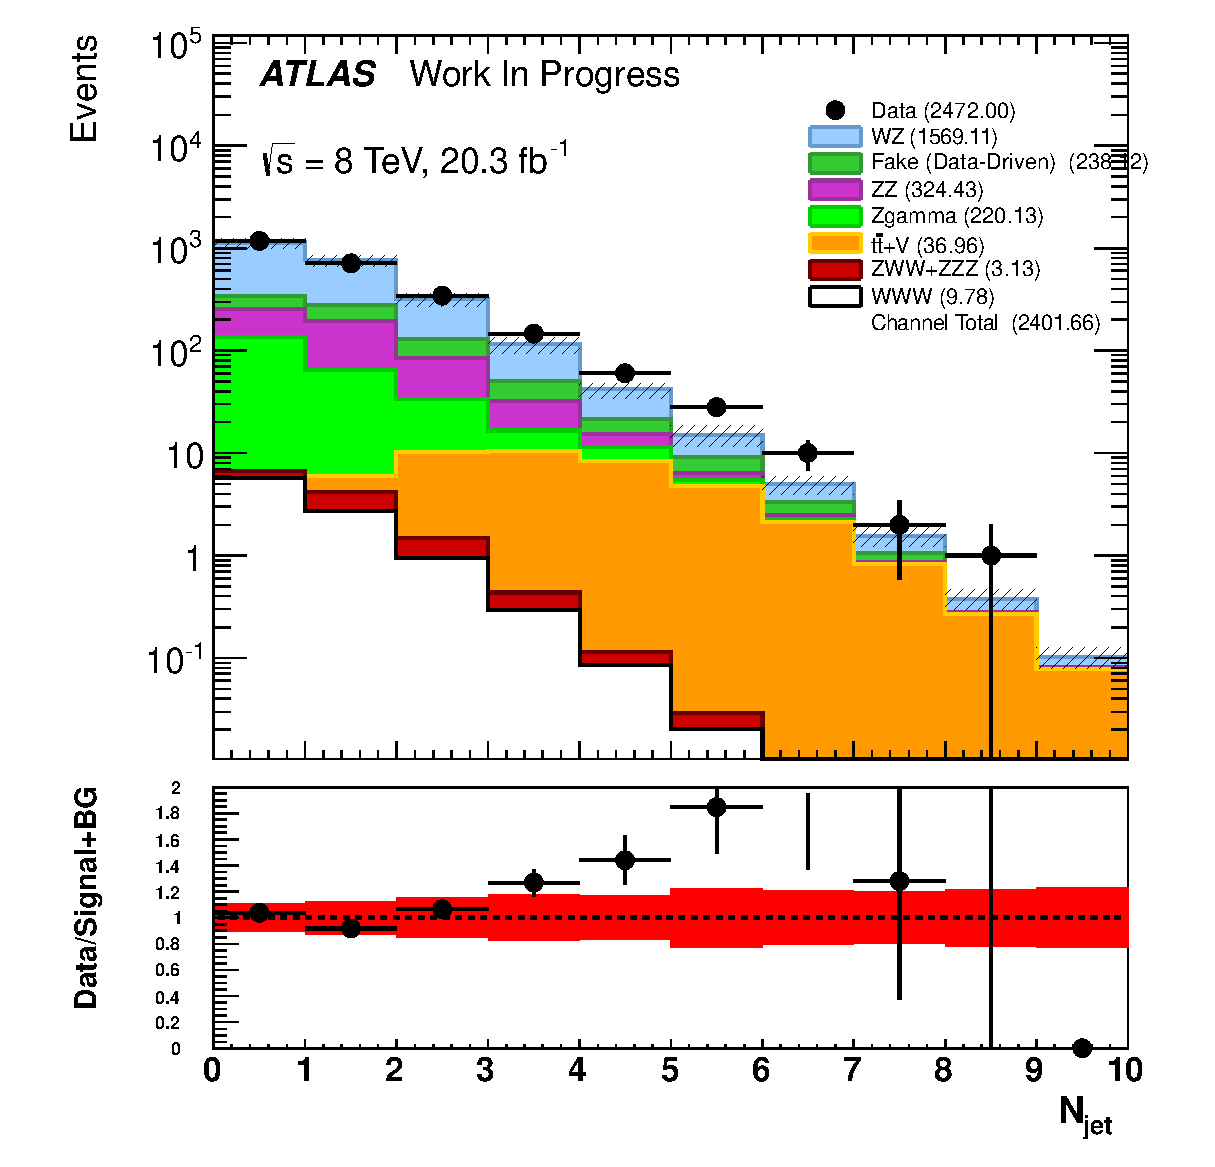
\includegraphics[width=0.3\columnwidth]{figures/appendix_signal_selection/Nov24Update_FakeSys_KFacSys_LogY_NoRebin/output/jobs/MxM/DataFull_Rates_May13_FakeRatesExactly2Loose_MuonMxMBJetGt0_ElBJetGt0SubtractPC_MxM/PreselectionNov23_15_physics/weight_all/eps/NJets_histratio.eps}
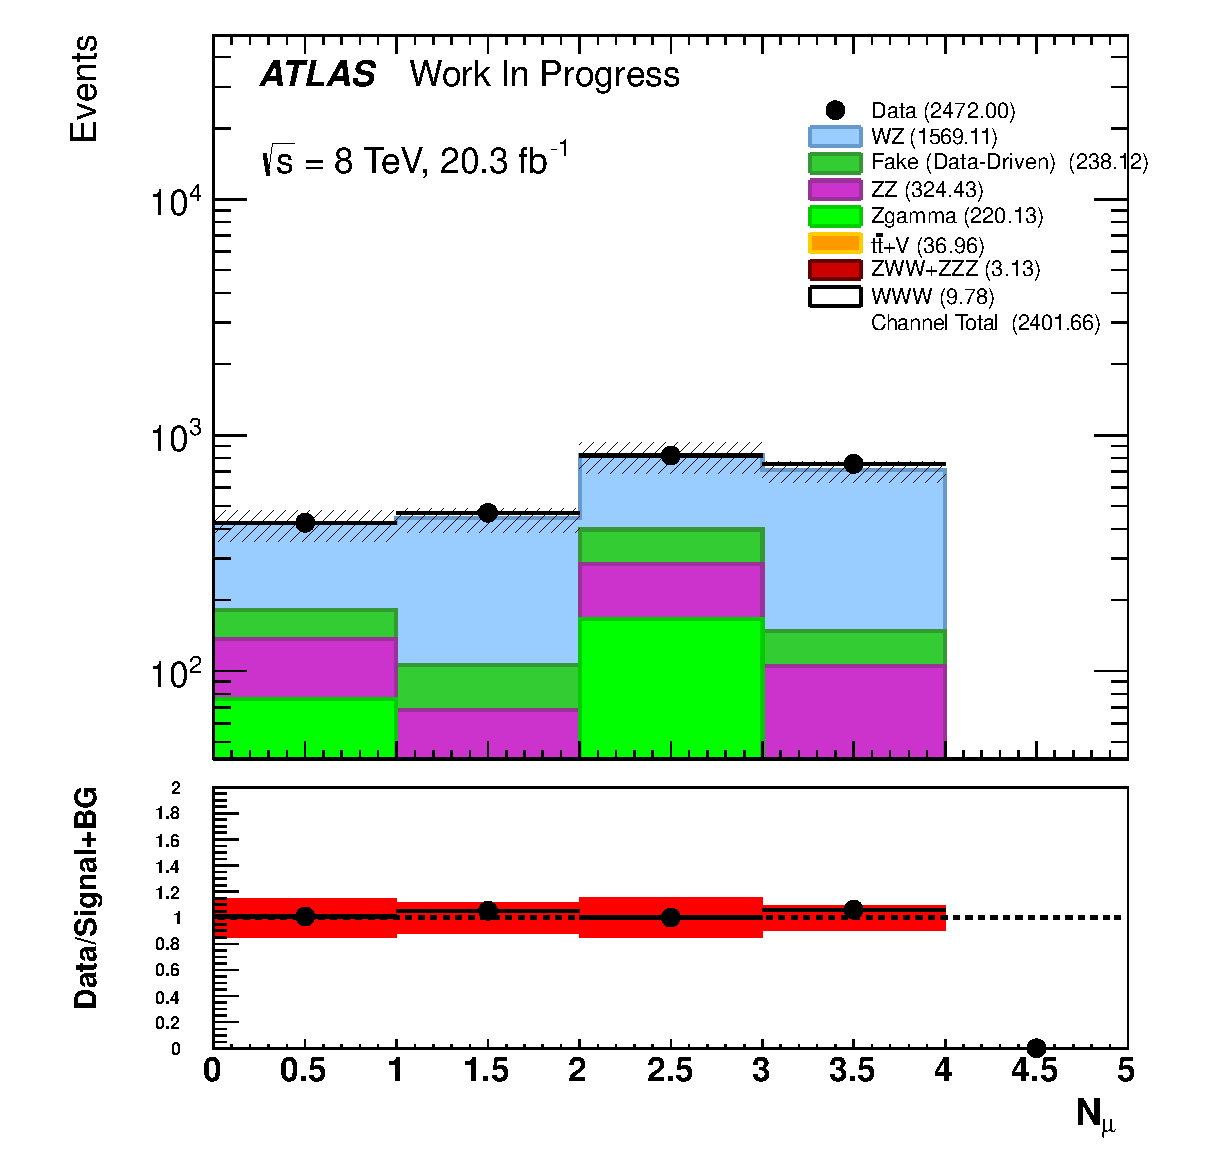
\includegraphics[width=0.3\columnwidth]{figures/appendix_signal_selection/Nov24Update_FakeSys_KFacSys_LogY_NoRebin/output/jobs/MxM/DataFull_Rates_May13_FakeRatesExactly2Loose_MuonMxMBJetGt0_ElBJetGt0SubtractPC_MxM/PreselectionNov23_15_physics/weight_all/eps/NMuons_histratio.eps}
%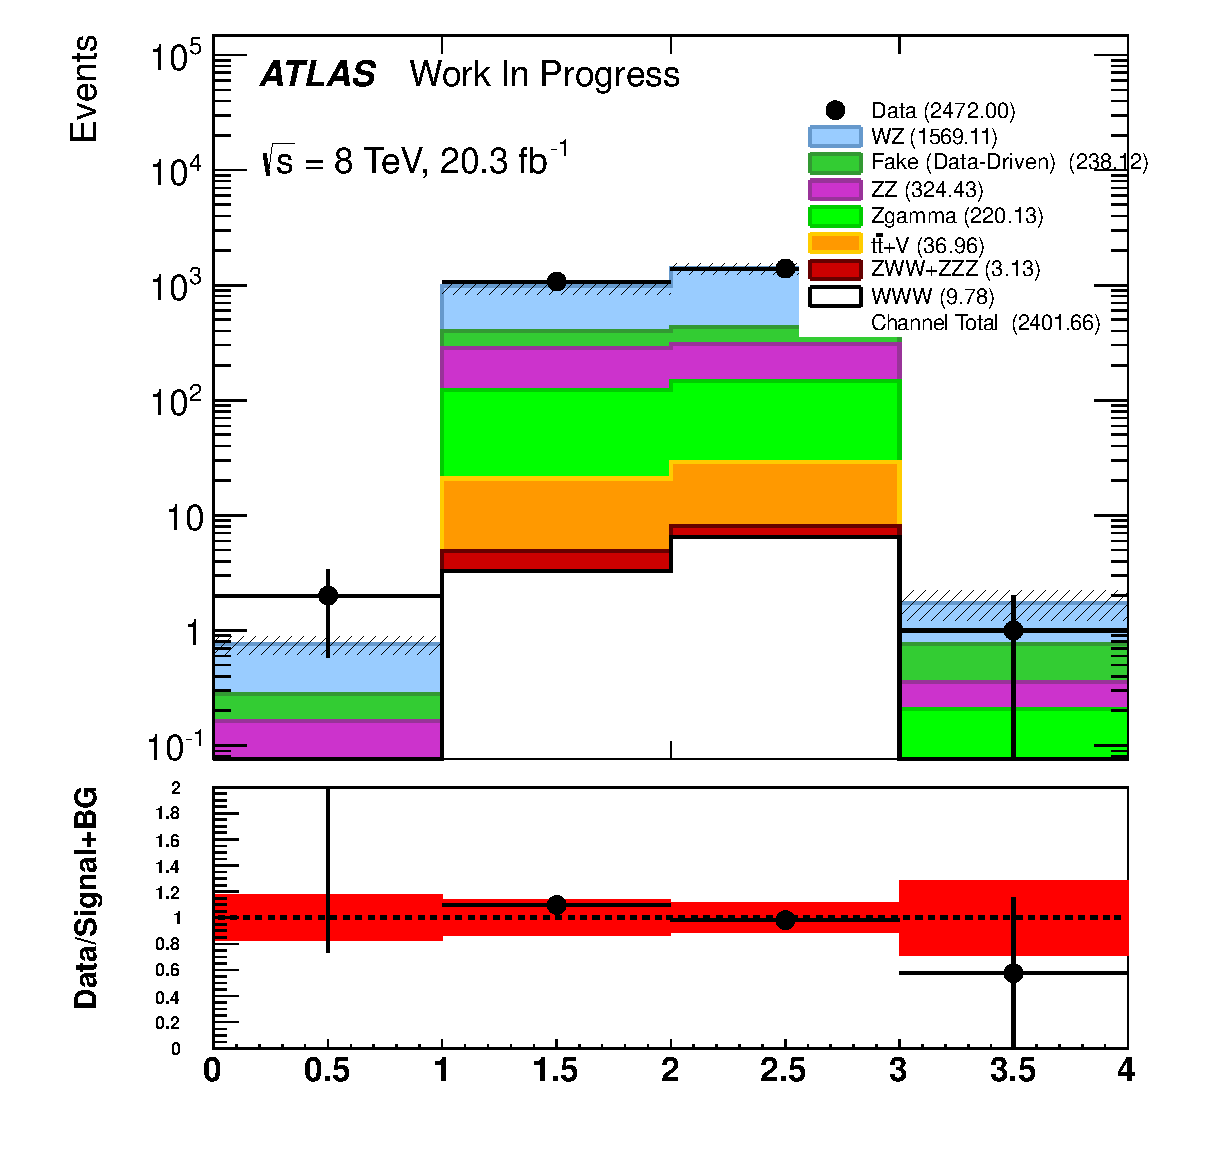
\includegraphics[width=0.3\columnwidth]{figures/appendix_signal_selection/Nov24Update_FakeSys_KFacSys_LogY_NoRebin/output/jobs/MxM/DataFull_Rates_May13_FakeRatesExactly2Loose_MuonMxMBJetGt0_ElBJetGt0SubtractPC_MxM/PreselectionNov23_15_physics/weight_all/eps/TotalCharge_histratio.eps}
\caption{Distributions showing the observed data compared to the background estimate at event pre-selection.}
\label{fig:preselection}
\end{figure}
The signal plus background model is compared to data at pre-selection
for a few different kinematic distributions of interest 
in \fig\ref{fig:preselection}. In the upper plot of each distribution,
the colored histograms 
represent the different categories contributing to the signal 
plus background model and 
are split by color into differnt categories based on the type of 
background and if it is the signal.  
%The colors are...
Hashed bands are shown on the stacked
histograms representing the size of the systematic uncertainties 
on the model, described later in \sec\ref{}.
The data is shown in the black points where the 
bars on the points represent the statistical uncertainty on the data.
The lower plot shows the ratio of the data over the model
In this case, the error bars correspond to the statistical uncertainty
on the ratio due to both the data and the model. The red band
shows the size of the systematic uncertainties with respect to the model.
The model is said to be consistent with the data
if the ratio is consistent with unity after considering statistical
and systematic uncertainties.
The different distributions are chosen primarly because 
of their potential to discriminate between signal and background. 
From top to bottom and left to right,
these distributions are: 
\begin{itemize}
\item Lepton $P_{T}^{1}$:  The momentum of the lepton in the transverse plane
which has the largest transverse momentum out of all three leptons selected.
\item Lepton $P_{T}^{2}$:  The momentum of the lepton in the transverse plane
which has the second largest transverse momentum out of all three leptons selected.
\item Lepton $P_{T}^{3}$:  The momentum of the lepton in the transverse plane
which has the smallest transverse momentum out of all three leptons selected.
\item $E_{T}^{Miss}$:  The missing transverse energy
\item $\Delta\varphi(lll,E_{T}^{Miss})$:  The difference in the polar angle 
between the three lepton $p_{T}$, 
$\overrightarrow{p_{T}^{lll}} =  \overrightarrow{p_{T}^{1}}+ 
\overrightarrow{p_{T}^{2}}+ \overrightarrow{p_{T}^{2}}$, 
and $E_{T}^{Miss}$. It can be expressed as 
$\Delta\varphi(lll,E_{T}^{Miss}) = \cos^{-1}\frac{ \overrightarrow{p_{T}^{lll}}\cdot\overrightarrow{E_{T}^{Miss}} }{ p_{T}^{lll}E_{T}^{Miss} } $
\item SFOS Invariant Mass ($m_{\textrm{SFOS}}$): The di-lepton invariant mass
of each SFOS lepton pair in the event. %do i need to define the invariant mass?
\item Three Lepton $m_{T}$: The transverse mass of the three lepton system
and the missing transverse energy, or
$m_{T}^{lll} = \sqrt{2p_{T}^{lll}E_{T}^{Miss}(1-\cos(\Delta\varphi(lll,E_{T}^{Miss})))}$ 
\item $N_{\textrm{Jet}}$: The number of jets selected in the event.
\item $N_{b-\textrm{Jet}}$: The number of $b$-jets tagged in the event.
\item $N_{\mu}$: The number of selected leptons that are muons. The maximum
possible is 3. If the lepton is not a muon it must be an electron.
\end{itemize}
In general, the signal plus background model is observed to be consistent
with the data at the pre-selection, at least for those distributions
considered here.



\subsection{Signal Region Selection}
\label{sec:signal_regions}
The signal regions used in this analysis are separated based on the number of 
Same-Flavor Opposite-Sign (SFOS) lepton pairs selected in the event.  That is to say,
the number of lepton pair combinations in the event 
which could feasibly come from the leptonic decay of a $Z$-boson.
This results in three separate signal regions listed 
below with the lepton charge combinations
which fall in each category:
\begin{itemize}
\item \textbf{0 SFOS}: $e^{\pm}e^{\pm}\mu^{\mp}$, 
$\mu^{\pm}\mu^{\pm}e^{\mp}$ ($e^{\pm}e^{\pm}\mu^{\pm}$, 
$\mu^{\pm}\mu^{\pm}e^{\pm}$, $e^{\pm}e^{\pm}e^{\pm}$, $\mu^{\pm}\mu^{\pm}\mu^{\pm}$)
\item \textbf{1 SFOS}: $e^{\pm}e^{\mp}\mu^{\pm}$, 
$e^{\pm}e^{\mp}\mu^{\mp}$, $\mu^{\pm}\mu^{\mp}e^{\pm}$, $\mu^{\pm}\mu^{\mp}e^{\mp}$
\item \textbf{2 SFOS}: $e^{\pm}e^{\pm}e^{\mp}$, $\mu^{\pm}\mu^{\pm}\mu^{\mp}$
\end{itemize}
Note that in the 2 SFOS region, one lepton is allowed to belong to both 
pair combinations.
Those combinations listed in parentheses are not allowed for the signal based on charge conservation (neglecting charge mis-identification).  
The amount of the $W^{\pm}W^{\mp}W^{\pm}$ signal
which falls into each category is purely combinatoric.  
From the above list one can thus see that there are twice as many ways 
for the signal combinations (again neglecting those in parentheses)
to fall in the 1 SFOS regions as 
there to fall in either the 0 SFOS or 2 SFOS regions. 
Absent possible differences in signal efficiencies based on the leptons in each 
signal region, one should expect branching 
fractions of 25\%, 50\% and 25\% for the 0, 1, and 2 SFOS signal regions, respectively.


\begin{figure}[ht!]
\centering
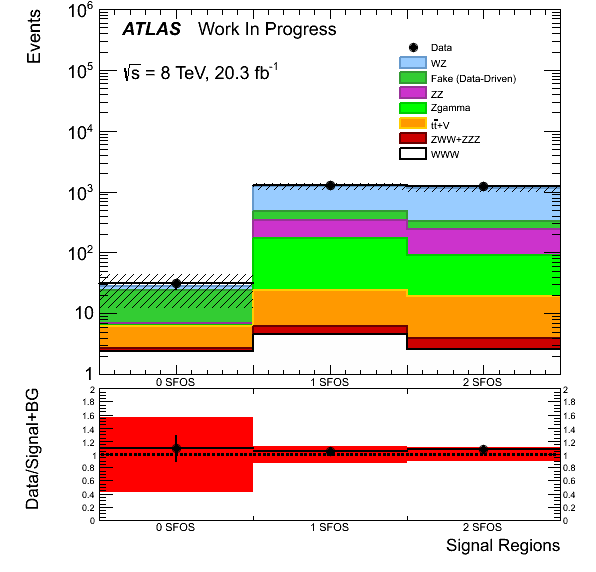
\includegraphics[width=0.5\columnwidth]{figures/SFOSPreselection.png}
\caption{Yields at event pre-selection in the 0, 1 and 2 SFOS regions.  
The most important systematic uncertainties 
(discussed in section~\ref{sec:systematics}) are shown, 
namely from the fake estimates and the uncertainties on the WZ and ZZ k-factors.}
\label{fig:preselection_nsfos}
\end{figure}

Indeed, upon splitting the preselection region based on the number of SFOS
pairs, we end up with signal and background predictions like in 
\fig\ref{fig:preselection_nsfos}, where we can see difference
in branching fraction for the signal to each of the three signal regions.
However, the most striking feature of this plot is the 
clear difference in background yield and background composition
between the 0 SFOS region and the 1 and 2 SFOS regions, which are similar.
Apparently, the advantage of splitting the signal region based on this
classification comes when looking at the background, specifically the
electroweak $WZ$ and $ZZ$ backgrounds where SFOS lepton pairs may be
produced from the decay of the $Z$ boson(s). Consider only the case
where the $WZ$ and $ZZ$ decay to either $e$ or $\mu$.  The $WZ$ production
process is thus characterized by 3 leptons with at least 1 SFOS lepton pair
which comes from the $Z$. If all three leptons from the $WZ$ decay have been
reconstructed, then the there is a 50~\% chance the third lepton 
will also be able to form a SFOS pair with one of the leptons from the $Z$ decay.
Thus, the WZ background will split evenly between the 1 and 2 SFOS classification.
Something similar occurs for the ZZ background except that the fourth lepton 
in the decay must be lost (usually due to possessing a low $\pt$).
The large cross-section for theses processes means that
they becomes the dominant backgrounds in the 1 and 2 SFOS regions.  
The 0 SFOS signal region is mostly spared from contamination  by 
these large processes but still
includes both the $WZ$ and $ZZ$ processes as background due to the
non-negligible (albeit small) effect of mis-measurement of the lepton
charge, see section~\ref{sec:chargeMisID}.  The 0 SFOS signal region
is thus unique in having a small background which is almost entirely
reducible and dominated instead by events where a jet is mis-measured
as or overlaps with a lepton, called the fake lepton background, along
with the aforementioned sub-dominant effect of lepton charge 
mis-identification described in Section~\ref{sec:chargeMisID}.  
From this, one can clearly see that it is
advantageous to split these signal regions so that the dominant
backgrounds in each region may be targeted individually.  Furthermore,
note that while the 1 SFOS region contains more of the signal than the
0 and 2 SFOS regions, it is the 0 SFOS region which is most likely to
have the best sensitivity due to the smaller background contribution.


Within each signal region it may be that we can further reduce the 
background with respect to the signal region. 
Because the background composition in the 0 SFOS region
is so different from the 1 and 2 SFOS regions, it is likely that
the selection which does this will also differ between them. 
And even though the
1 and 2 SFOS regions are resonably similar, we should not rule out
the possibility that they also have a uniquely optimial selection.
Based on heuristic arguments, a list of reasonable physical
quantities were considered. The most promising of these quantities
are those listed previously in \sec\ref{sec:preselection}. 
By restricting these quantities to a region which removes a larger
fraction of background than it does the signal, we can 
increase the signal prediction with respect to the background.
The ratio of events which pass a selection with respect
to the original number of events is refferred to as the 
efficiency.
Thus, we refer to this process 
as choosing a selection threshold where 
the signal efficiency is larger than the background efficiency.
Consider the following selection choices using the quantities defined
earlier:
%Do I need to add more plots here???
\begin{itemize}
\item Lepton $P_{T}$:  Require that exactly three leptons passing tight object quality requirements have a $P_{T} > X$.
\item Missing $E_{T}$:  Require that $E_{T}^{Miss} > X$.
\item $\Delta\varphi(lll,E_{T}^{Miss})$:  Require that $\Delta\varphi(lll,E_{T}^{Miss}) = \cos^{-1}\frac{ \overrightarrow{p_{T}^{lll}}\cdot\overrightarrow{E_{T}^{Miss}} }{ p_{T}^{lll}E_{T}^{Miss} } > X$.
\item Jet Veto: Require that $N_{Jet} \leq X$.
\item b-Jet Veto: Require that $N_{b-Jet} \leq X$.
%\item Z Veto: Require that $m_{ll}$ does not fall in the region $m_{Z}-m_{min} < m_{ll} < m_{Z}-m_{max}$ where $m_Z = 91.1876$~GeV and where $m_{min}$ are $m_{max}$ are the boundaries of the Z-window with which to veto.  For the 1 and 2 SFOS regions the pairs used to construct the $m_{ll}$ are SFOS pairs of either electrons or muons.  In the 0 SFOS region there are no SFOS pairs by definition but there is still a Z-peak in the same-sign di-electron mass spectrum due to charge mis-id. Thus, in the 0 SFOS region we consider instead
same-sign electron pairs.
\item Three Lepton $m_{T}$: Require that $m_{T}^{lll} > X$
%\item Same-flavor mass: Consider cuts on $m_{SF} > m_{min}$ and/or $m_{SF} < m_{max}$ where $m_{SF}$ is the invariant mass of same-flavor pairs (with no requirement on the sign) %what about this one?
\end{itemize}


\begin{figure}[ht!]
\centering
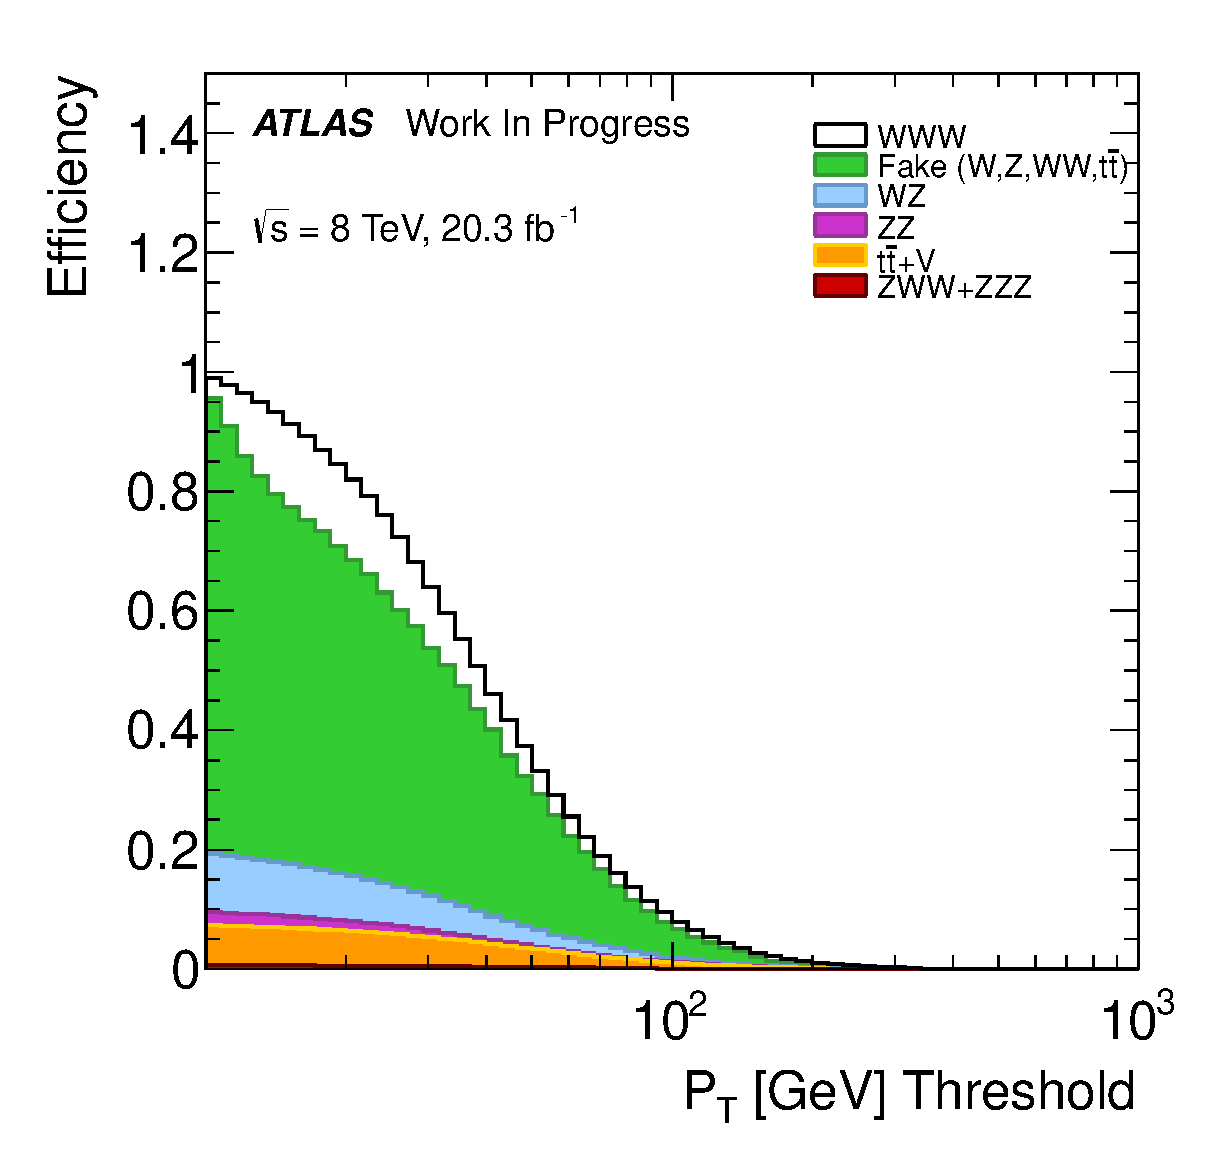
\includegraphics[width=0.3\columnwidth]{figures/optimization/SignalRegionsPreselection_0SFOS_Efficiencies/AllLeptonPt_Cumulative.eps}
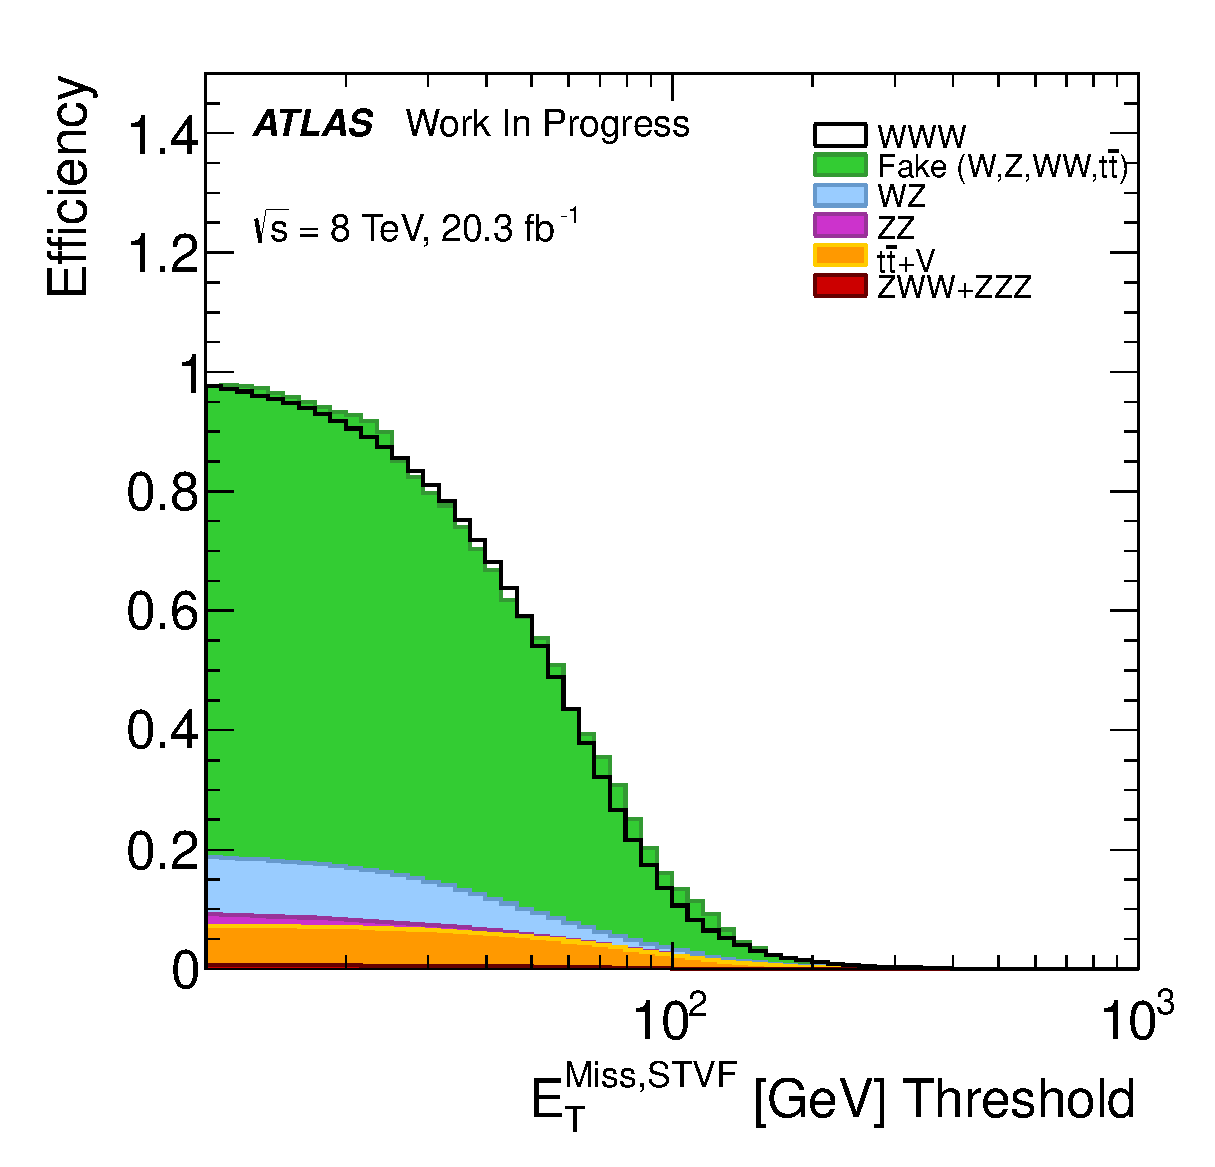
\includegraphics[width=0.3\columnwidth]{figures/optimization/SignalRegionsPreselection_0SFOS_Efficiencies/MET_Et_STVF_Cumulative.eps}
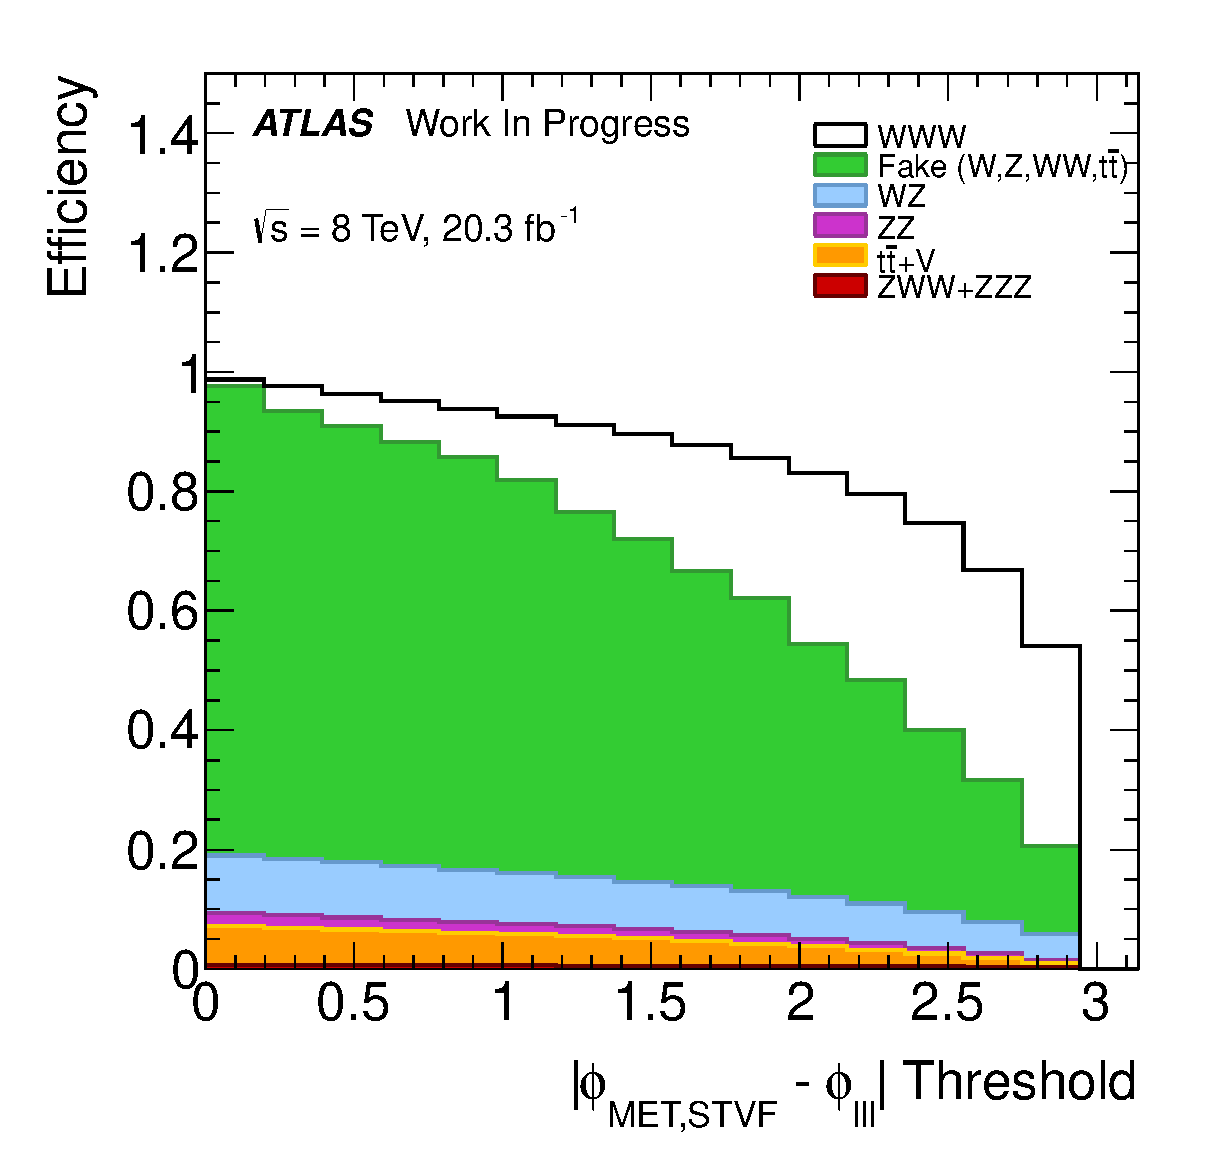
\includegraphics[width=0.3\columnwidth]{figures/optimization/SignalRegionsPreselection_0SFOS_Efficiencies/DeltaPhiMETSTVF123_Abs_Cumulative.eps}
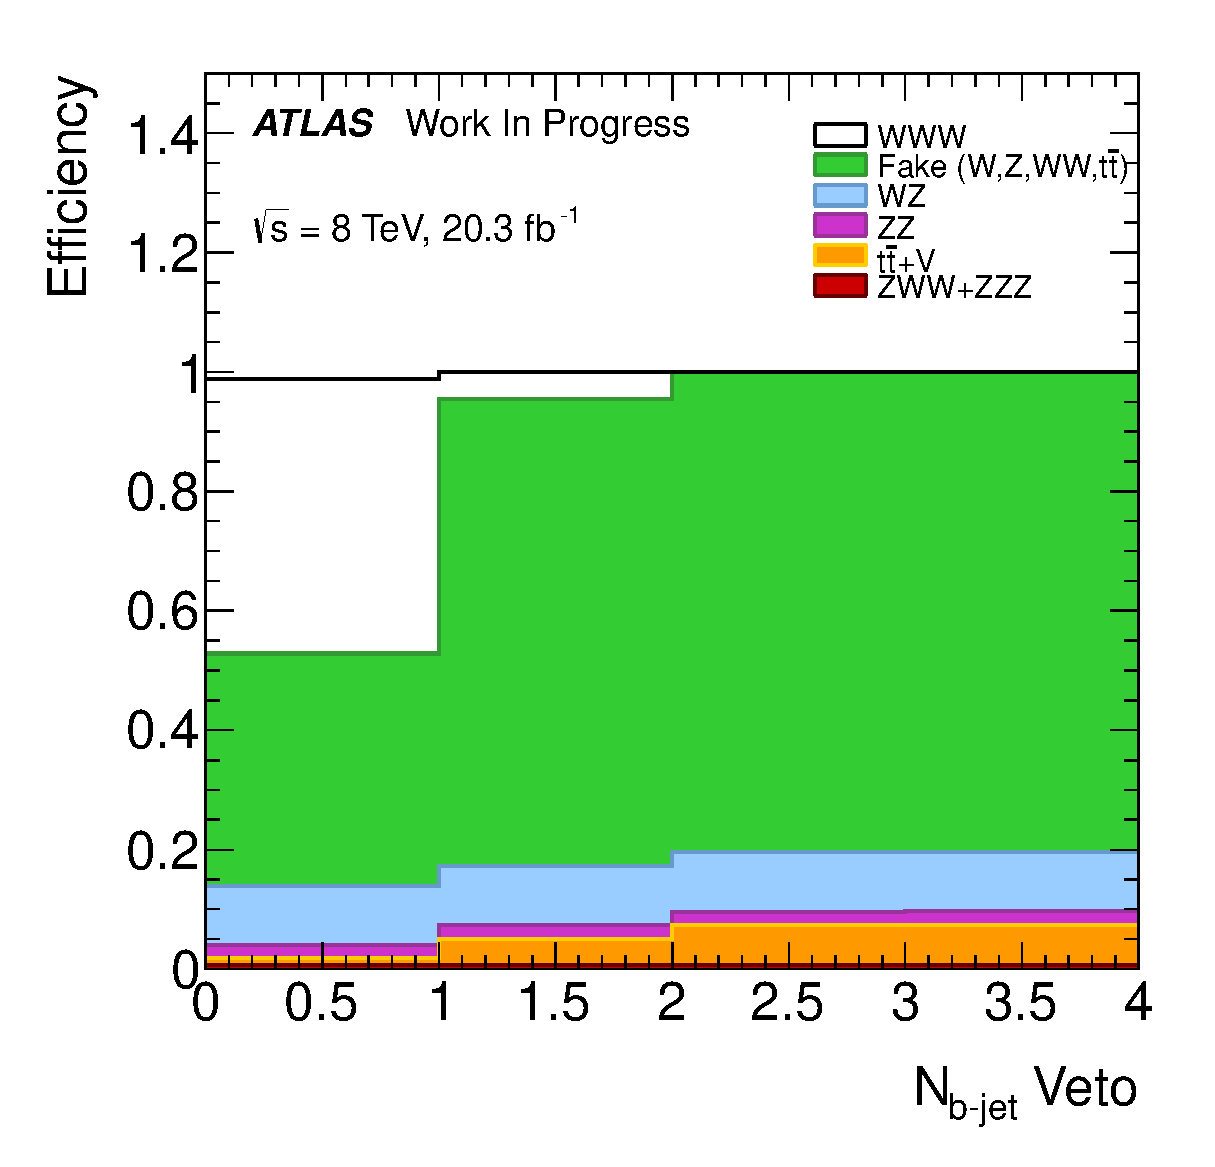
\includegraphics[width=0.3\columnwidth]{figures/optimization/SignalRegionsPreselection_0SFOS_Efficiencies/NBTaggedJets_LeftCumulative.eps}
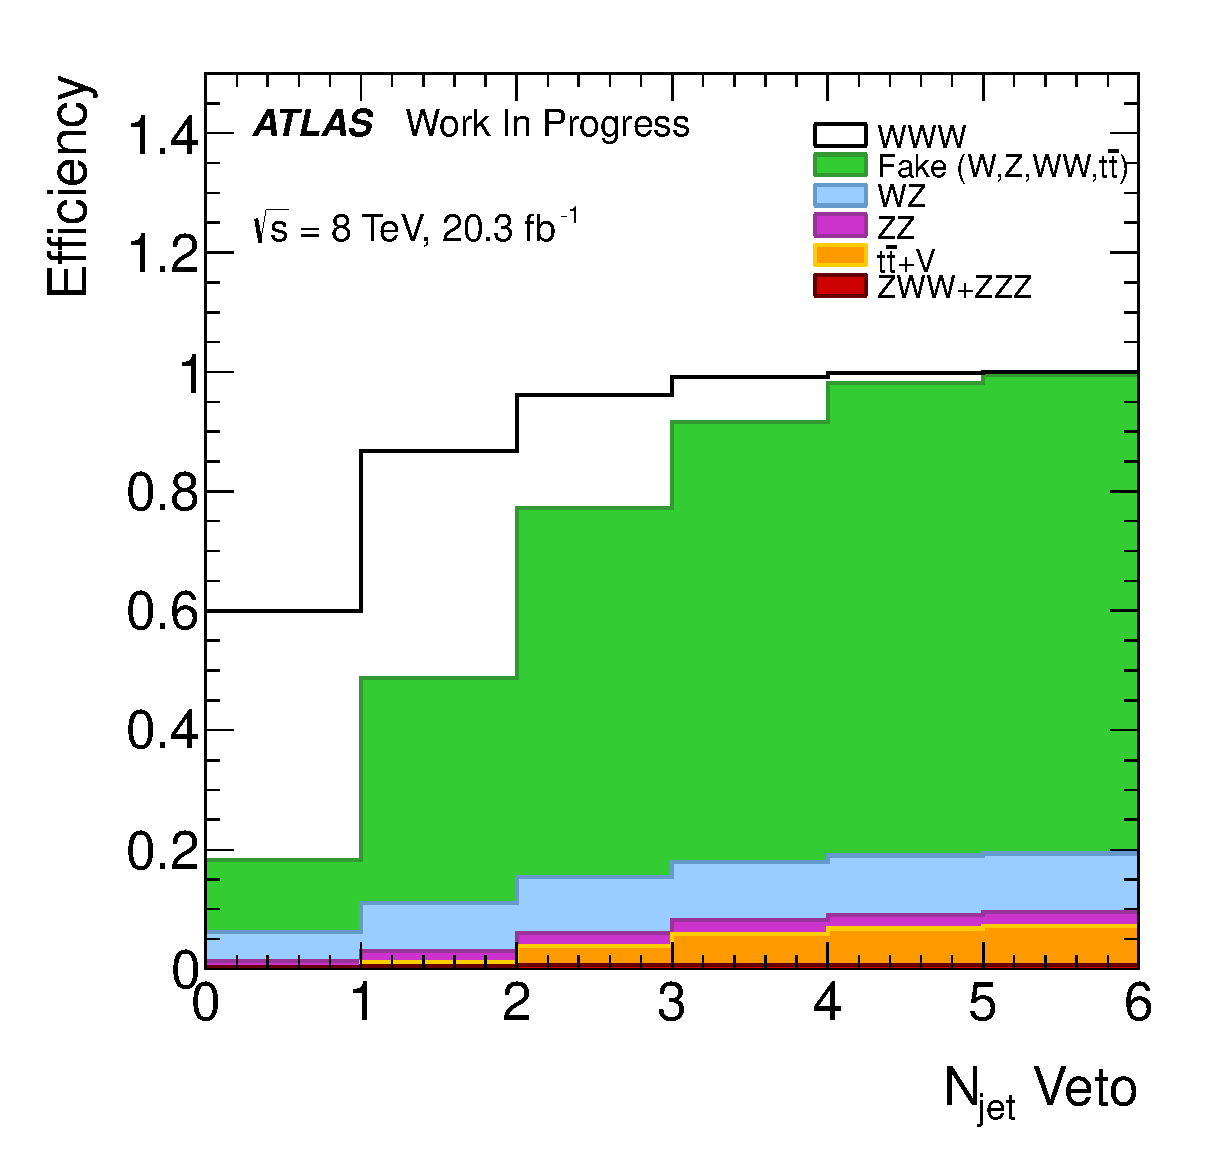
\includegraphics[width=0.3\columnwidth]{figures/optimization/SignalRegionsPreselection_0SFOS_Efficiencies/NJets_LeftCumulative.eps}
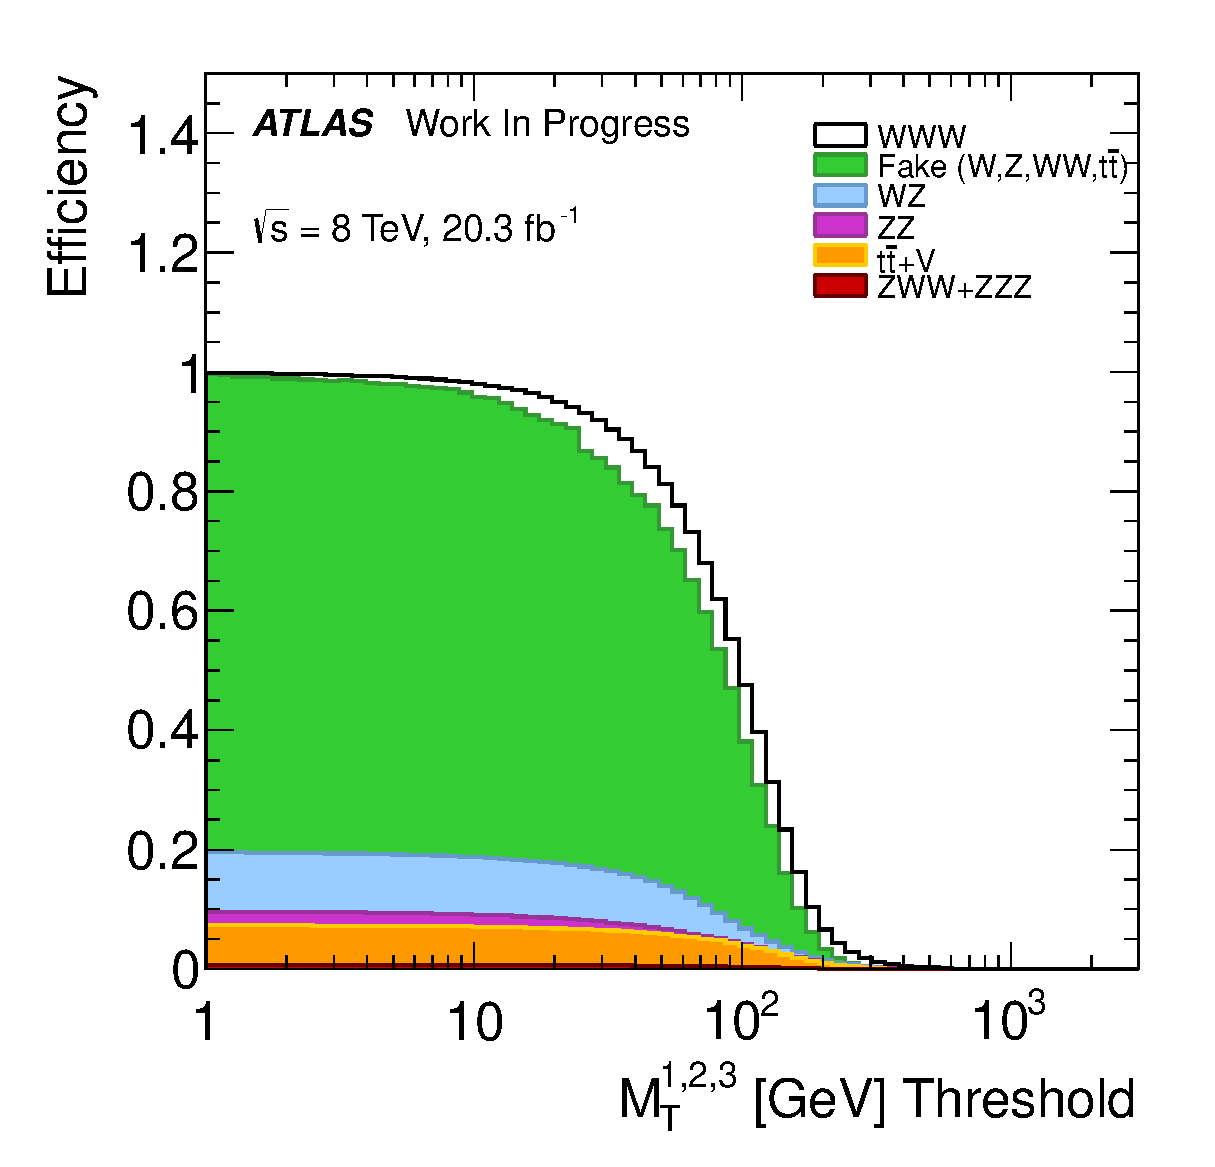
\includegraphics[width=0.3\columnwidth]{figures/optimization/SignalRegionsPreselection_0SFOS_Efficiencies/ThreeLeptonMt_Cumulative.eps}
%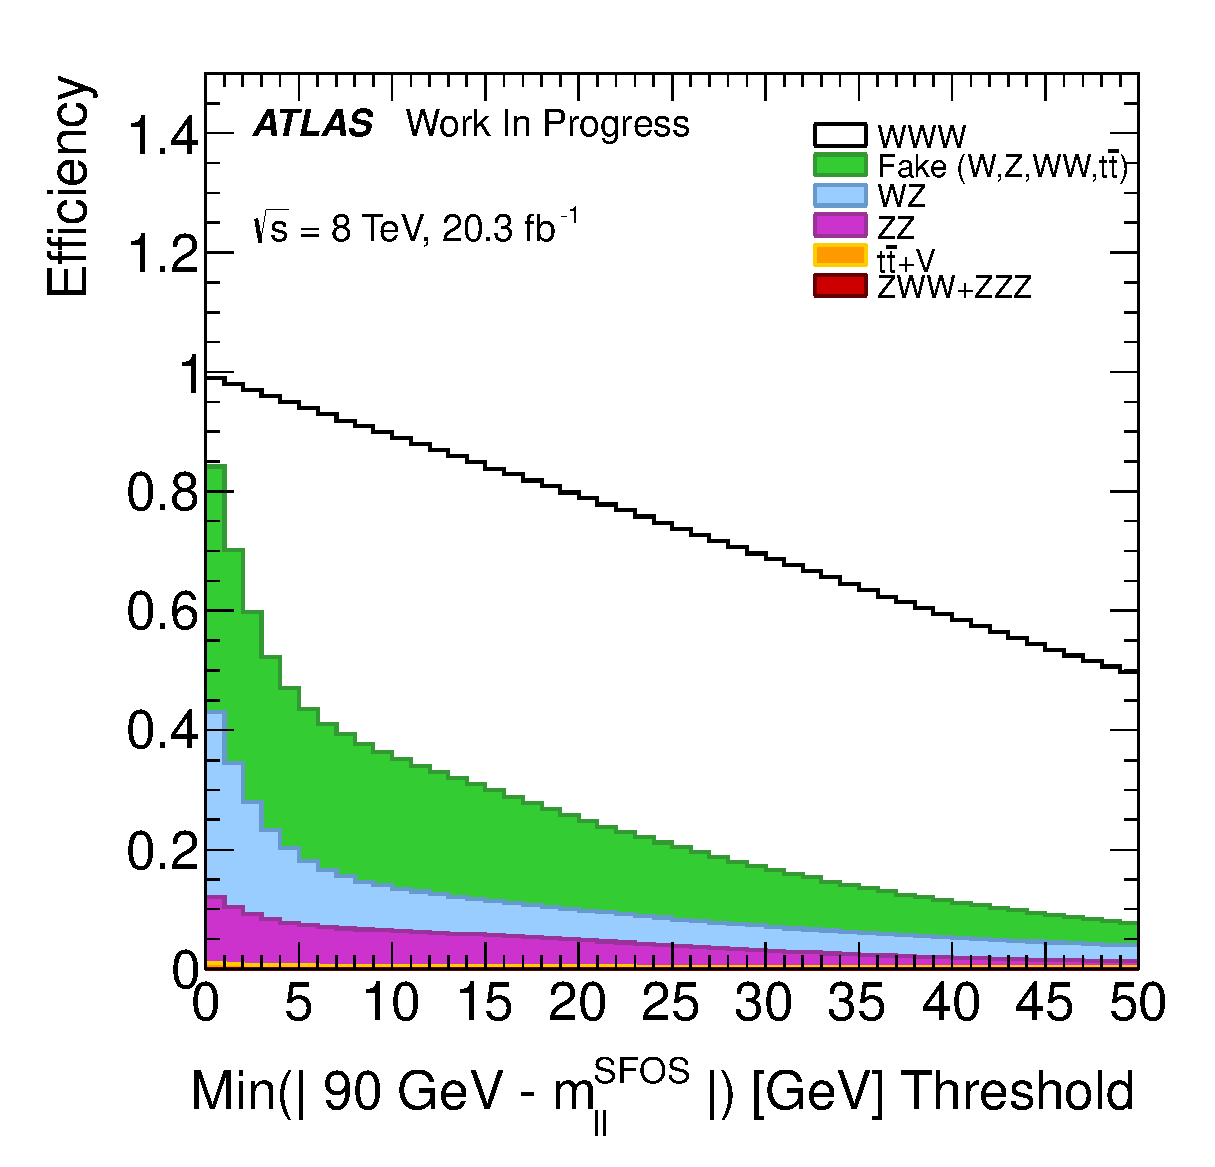
\includegraphics[scale=0.25]{figures/optimization/SignalRegions_0p5mmZ0_Preselection_Efficiencies/ZWindow_Cumulative.eps}
\caption{Signal and background efficiencies as a function of various cuts when starting from event pre-selection + 0 SFOS lepton pairs.}
\label{fig:optimization_efficiencies_0sfos}
\end{figure}

\begin{figure}[ht!]
\centering
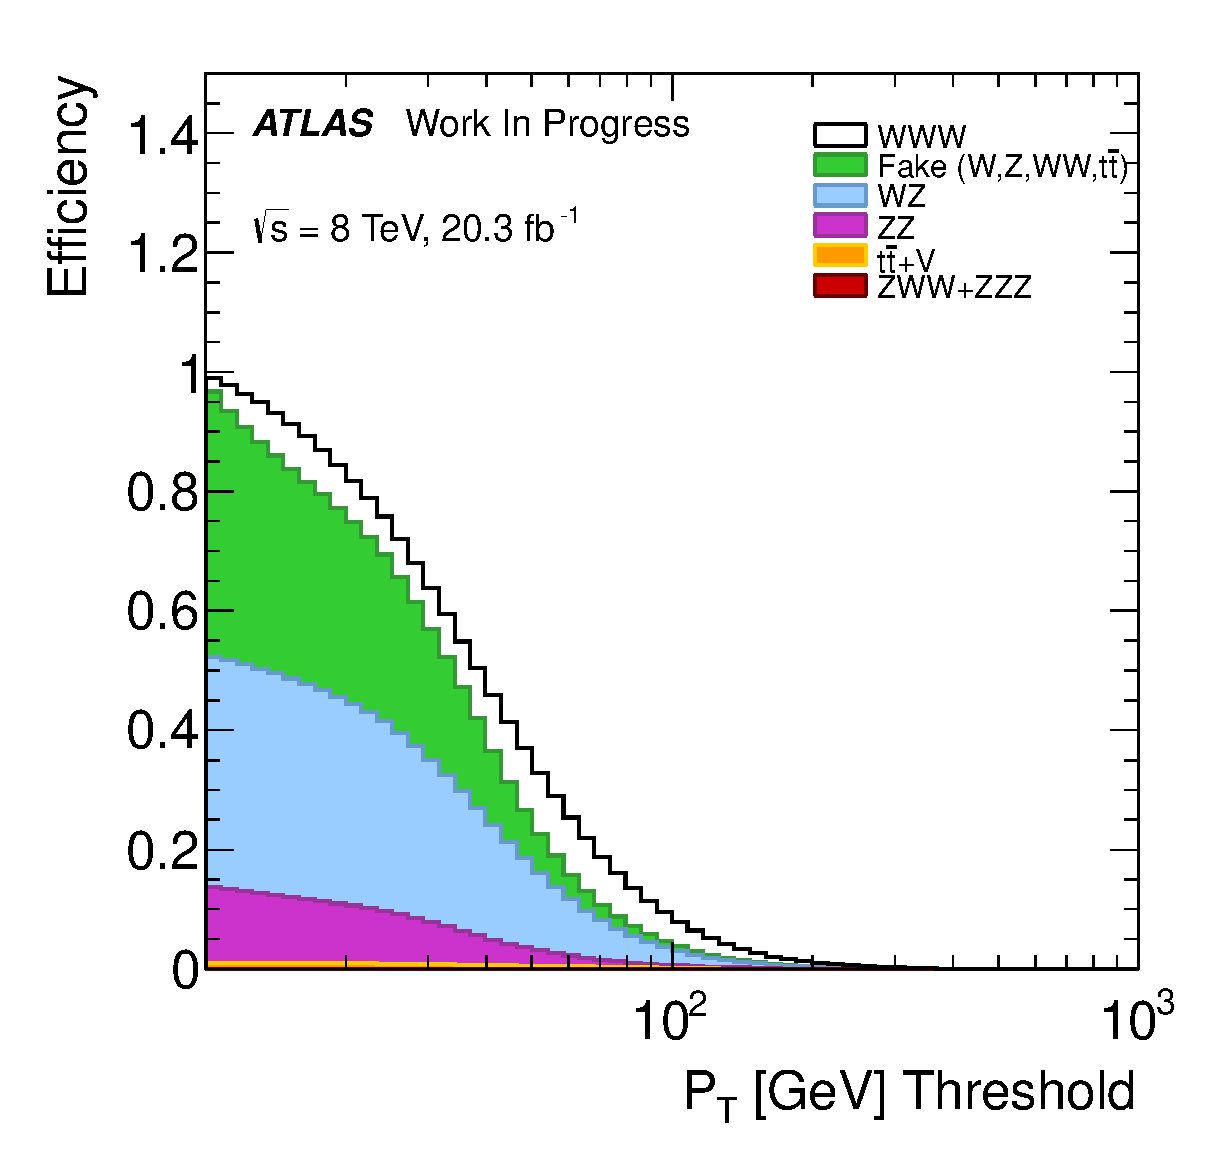
\includegraphics[width=0.3\columnwidth]{figures/optimization/SignalRegions_0p5mmZ0_Preselection_Efficiencies/AllLeptonPt_Cumulative.eps}
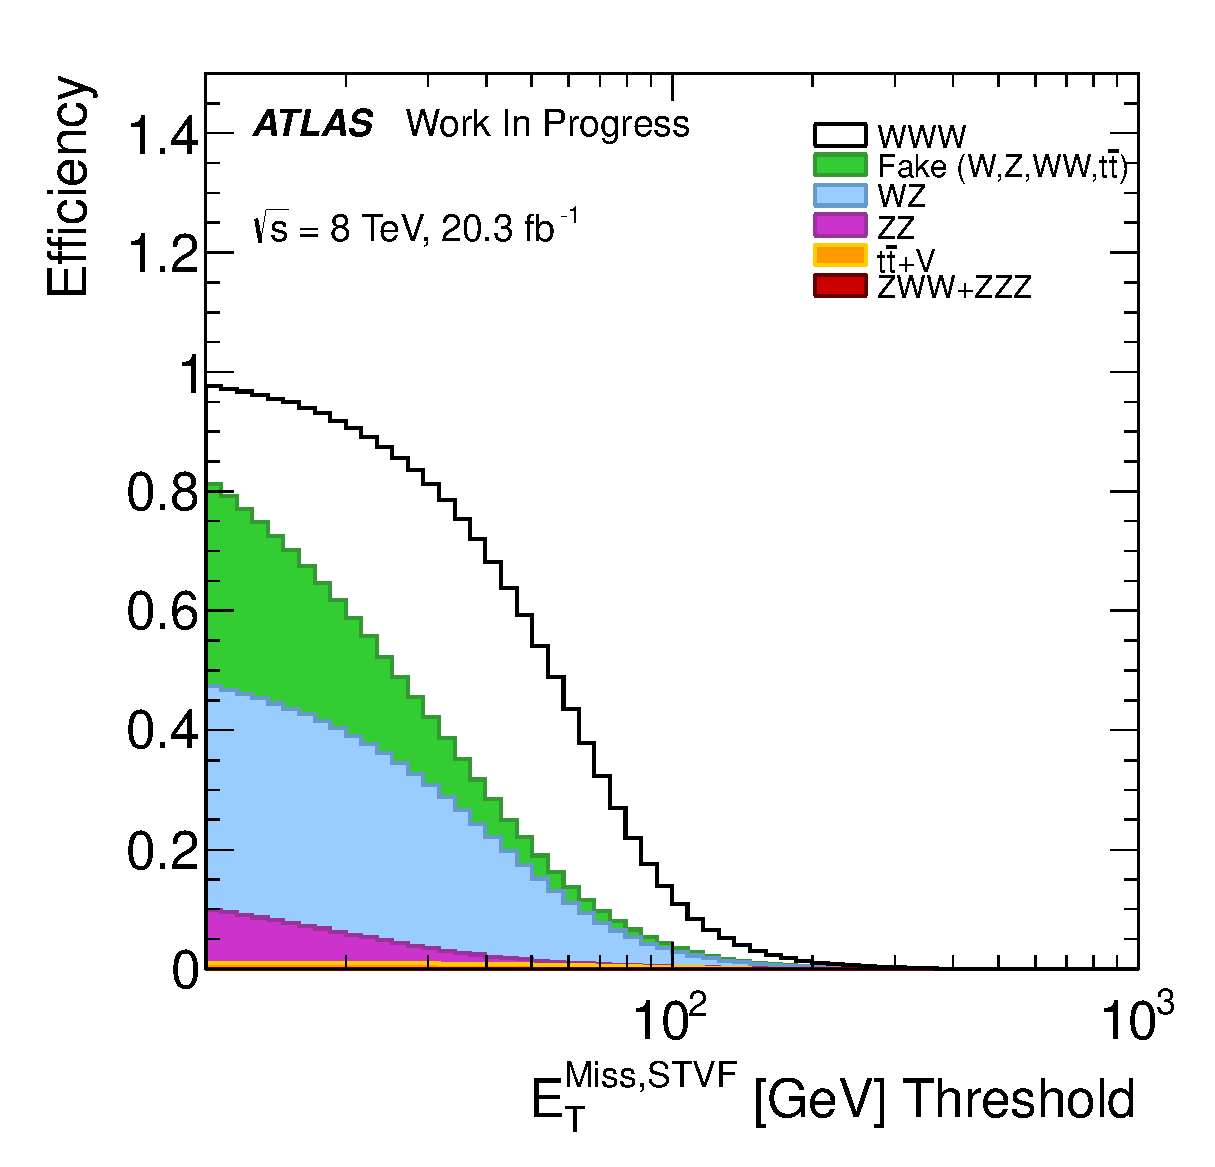
\includegraphics[width=0.3\columnwidth]{figures/optimization/SignalRegions_0p5mmZ0_Preselection_Efficiencies/MET_Et_STVF_Cumulative.eps}
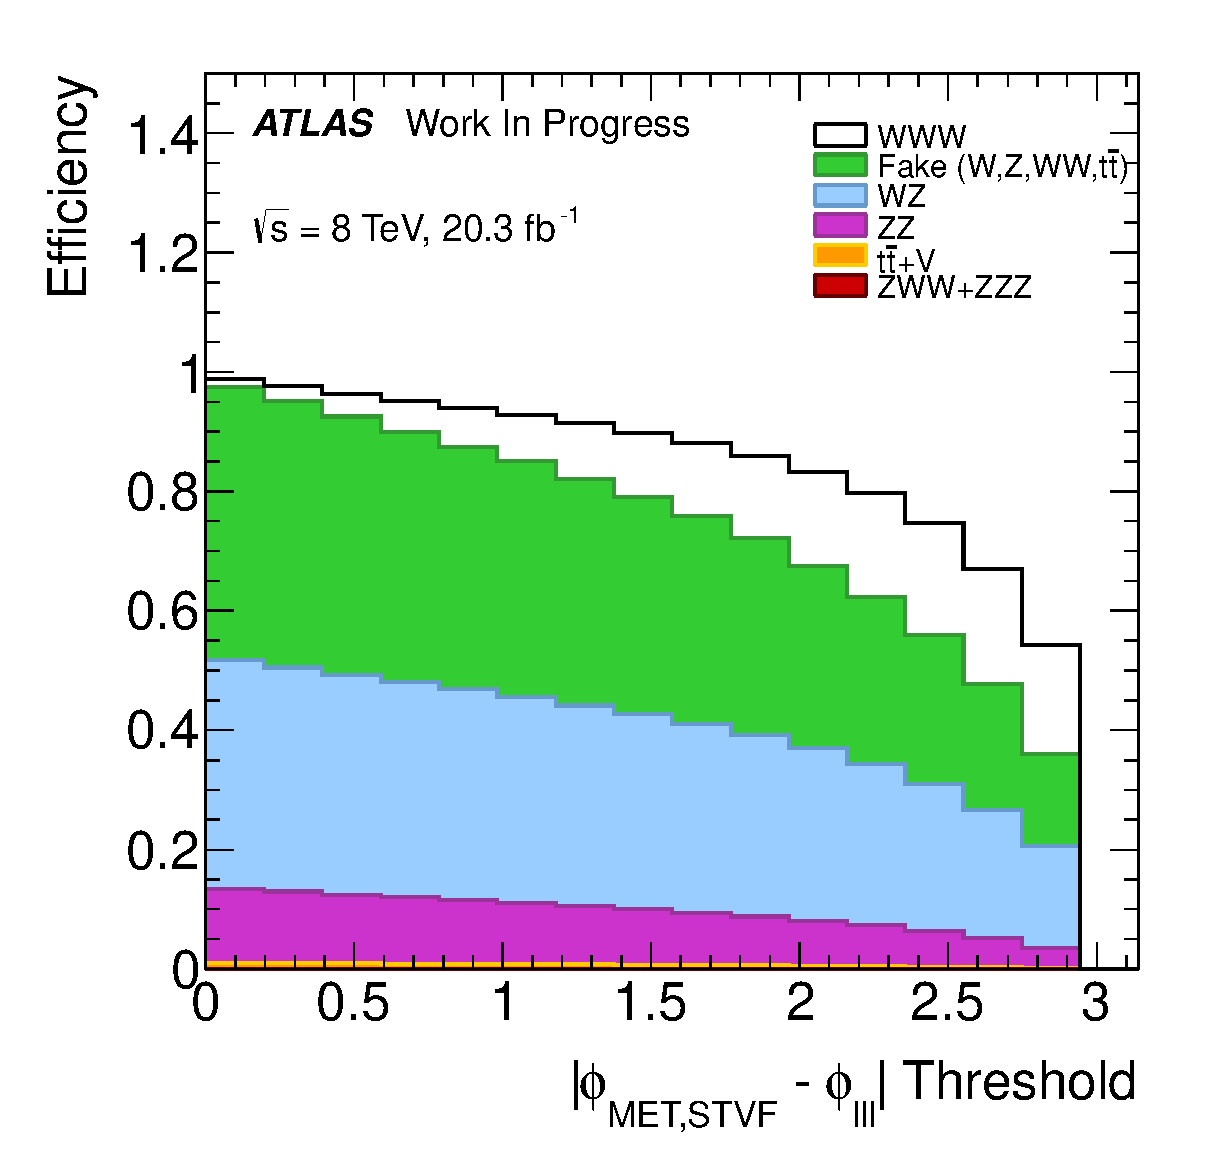
\includegraphics[width=0.3\columnwidth]{figures/optimization/SignalRegions_0p5mmZ0_Preselection_Efficiencies/DeltaPhiMETSTVF123_Abs_Cumulative.eps}
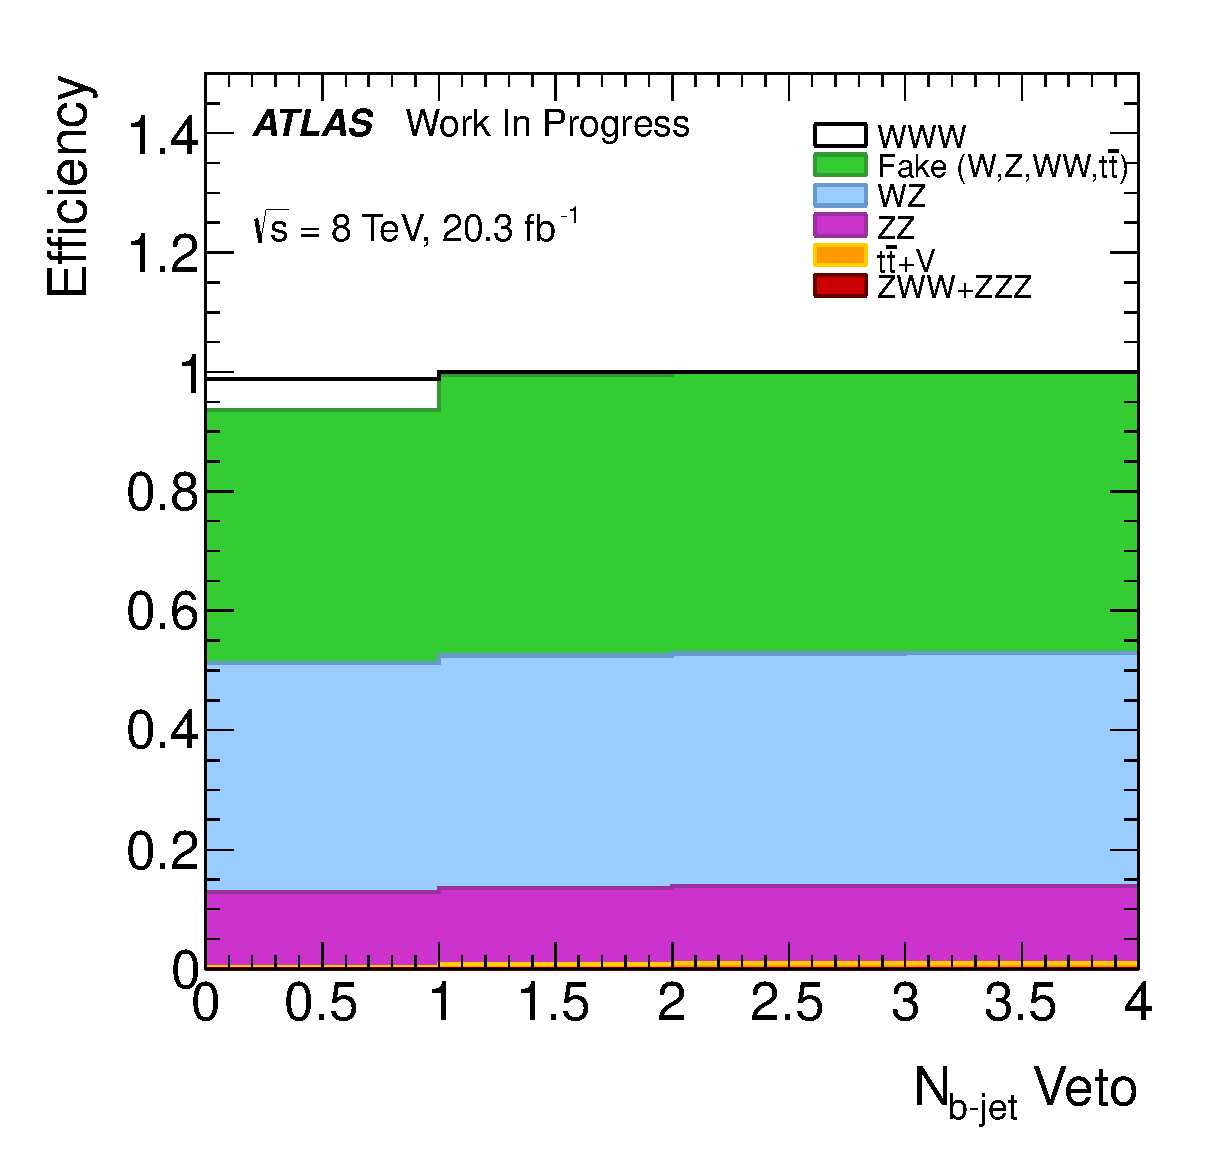
\includegraphics[width=0.3\columnwidth]{figures/optimization/SignalRegions_0p5mmZ0_Preselection_Efficiencies/NBTaggedJets_LeftCumulative.eps}
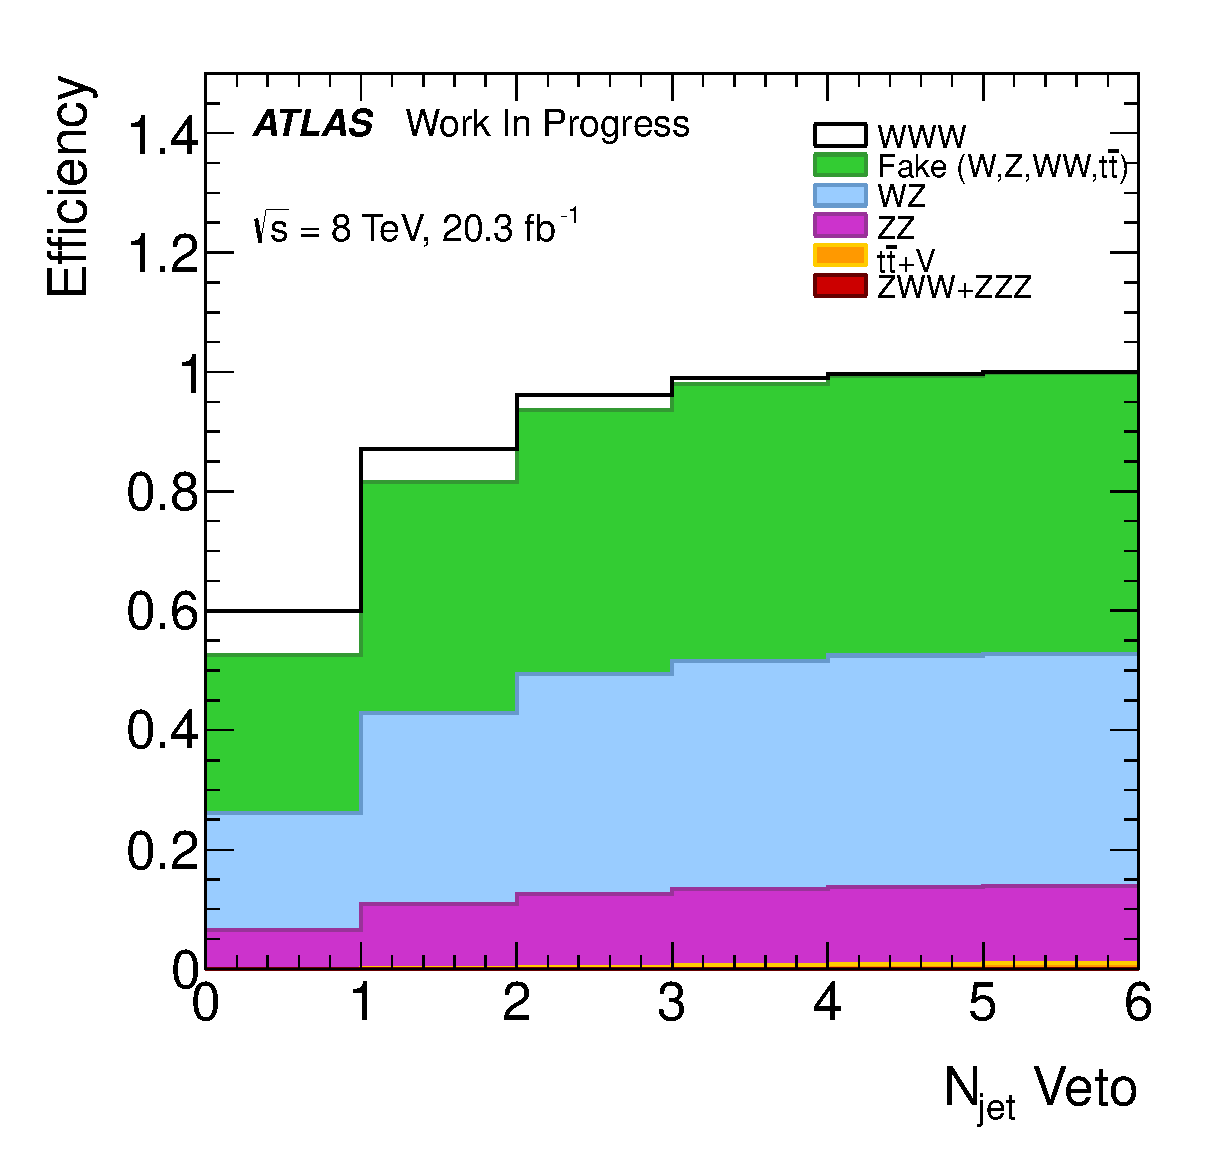
\includegraphics[width=0.3\columnwidth]{figures/optimization/SignalRegions_0p5mmZ0_Preselection_Efficiencies/NJets_LeftCumulative.eps}
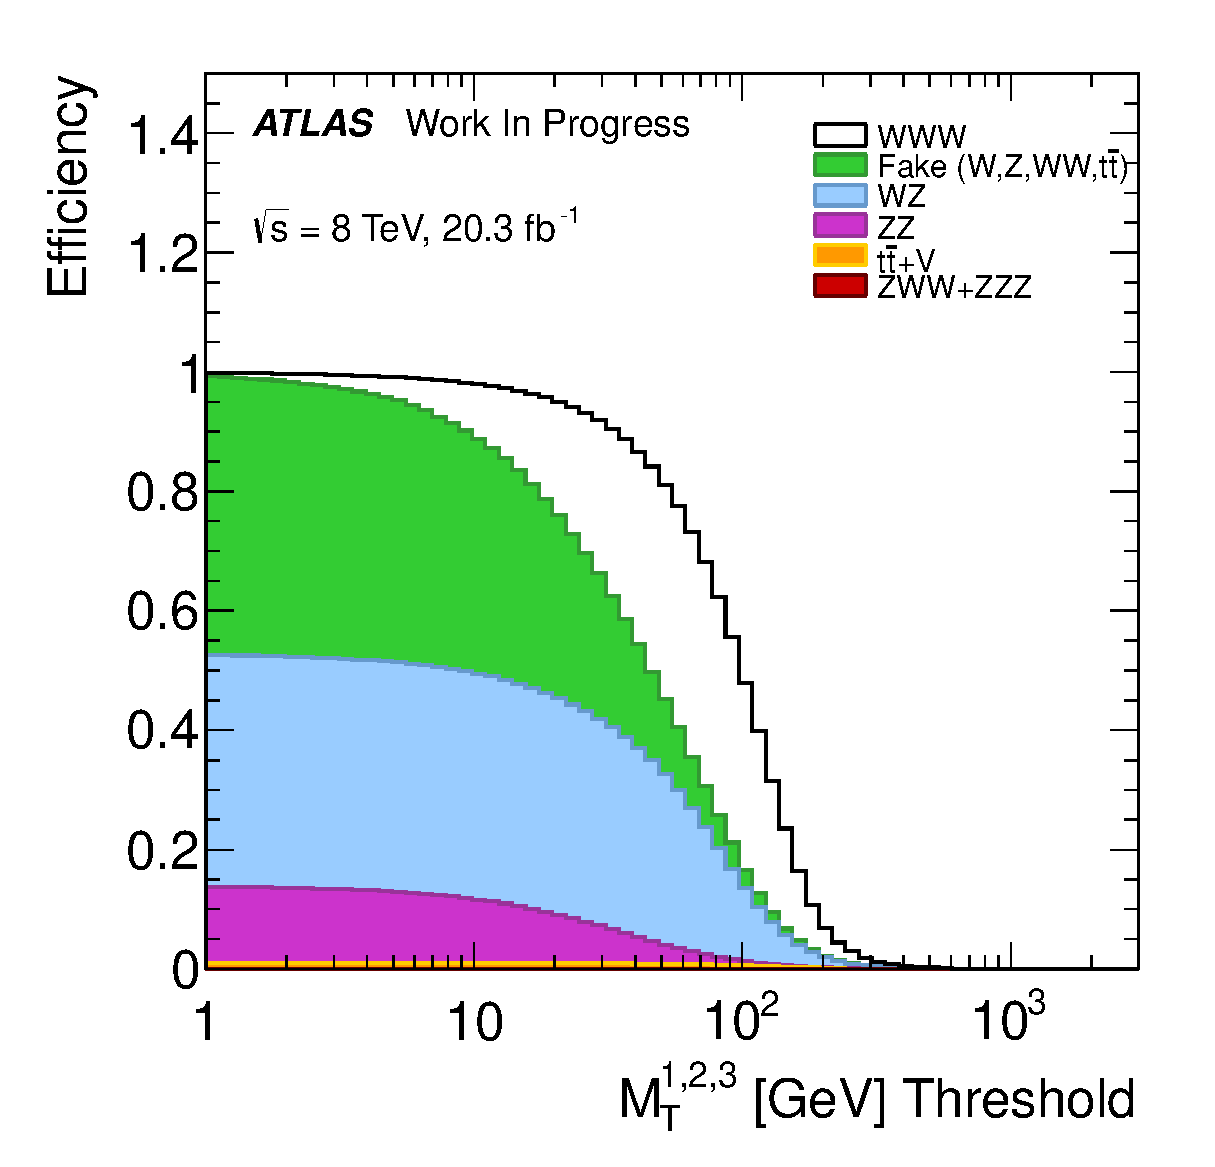
\includegraphics[width=0.3\columnwidth]{figures/optimization/SignalRegions_0p5mmZ0_Preselection_Efficiencies/ThreeLeptonMt_Cumulative.eps}
%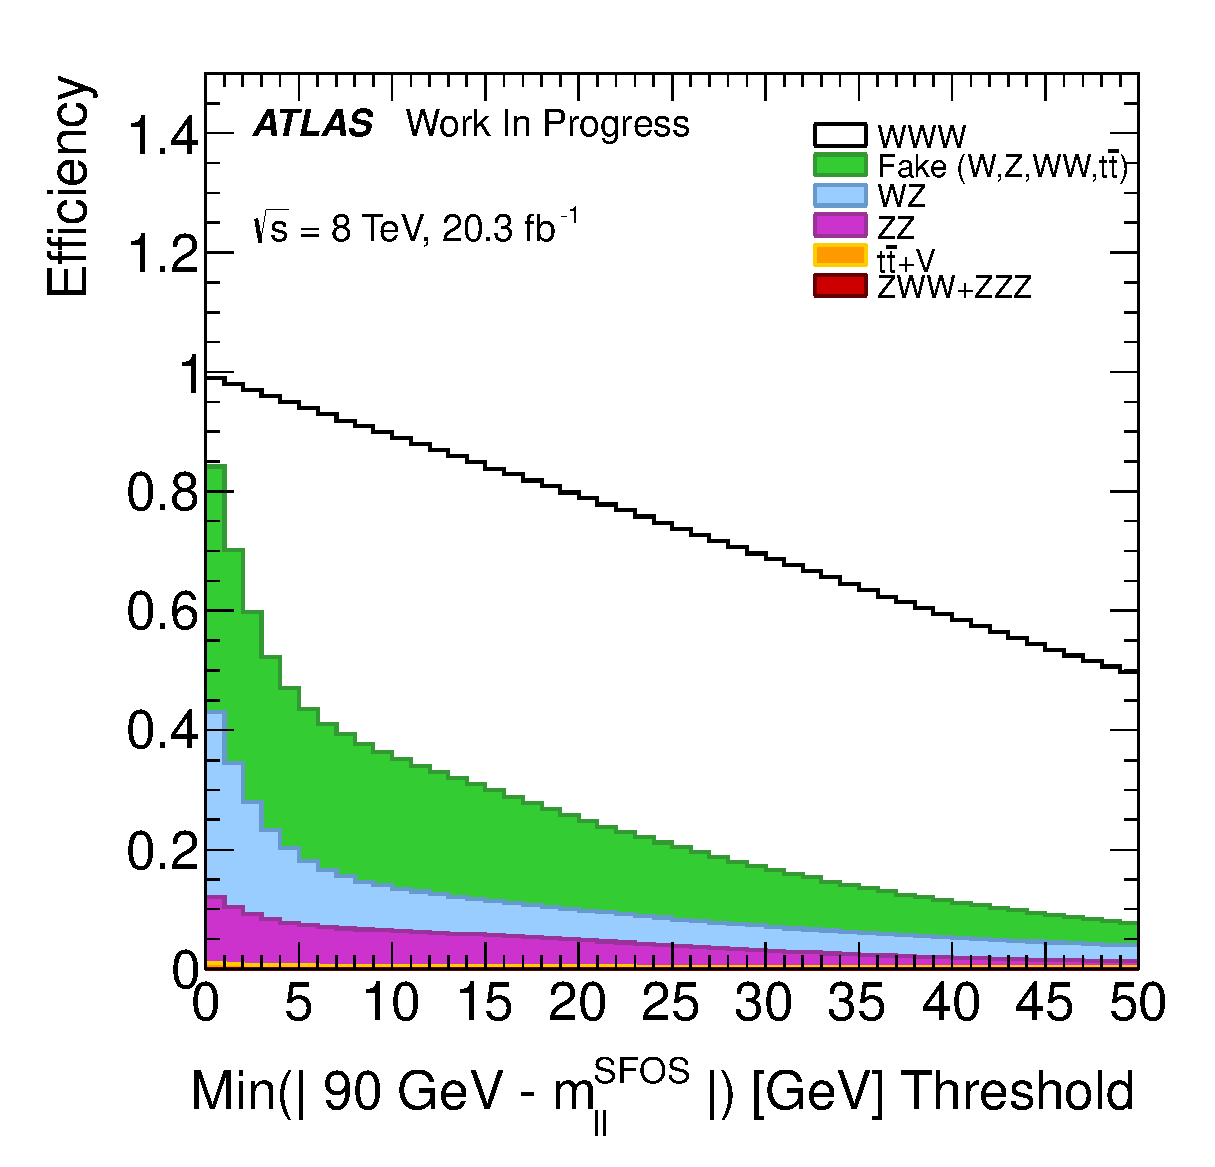
\includegraphics[scale=0.25]{figures/optimization/SignalRegions_0p5mmZ0_Preselection_Efficiencies/ZWindow_Cumulative.eps}
\caption{Signal and background efficiencies as a function of various cuts when starting from event pre-selection.}
\label{fig:optimization_efficiencies_preselection}
\end{figure}

We can plot the efficiency for the signal as well as the background
as a function of the threshold, $X$, for each of these quantities. 
The efficiencies are shown in the pre-selection + 0 SFOS region
in \fig\ref{fig:optimization_efficiencies_0sfos} and for
just the pre-selection region in 
\fig\ref{fig:optimization_efficiencies_preselection} (which
has a similar background composition to the 1 and 2 SFOS regions).
Clearly, the shape of the efficiencies between the signal and
background is not always the same, which means that we have some
power to reduce to background with respect to the signal.
Furthermore, these shapes are not the same in the pre-selection 
+ 0 SFOS region as they are in just the and pre-selection region.

For instance, in the 0 SFOS region, the shape of the efficiencies
for signal and background are very similar as a function
of the \MET~threshold, but in the pre-selection stage they are
very differerent, with the background efficiency dropping much
more rapidly than the signal efficiency. This suggests that
a cut on the \MET~distribution could be very useful 
in the 1 and 2 SFOS regions but not in the 0 SFOS region.

Other insights that can be gained from looking at these distributions
are that the \deltaphi~...


Correlations between these cuts mean that we should not make the final
selection decision based on these arguments alone. 
Instead, we use an optimization procedure...

STOP



It should be said that a more algorithmic way of choosing the type
of quantities to consider could improve this selection. Deep learning...





The final signal selection cuts are determined using an optimization
procedure which considers both the signal yield as well as the uncertainty
on the measurement (including statistical and systematic uncertainties)
of the signal strength as taken from the profile likelihood. 

Many different quantities were considered in the optimization.  All three signal 
regions start from event pre-selection (described above in Section~\ref{sec:preselection}) where 
we have 3 leptons with a $\pt$ of at least 20~GeV 
and where at least one of the leptons is matched to one of the single lepton triggers.
It was considered whether or not to lower the $\pt$ threshold, but this was found to increase
the fake lepton background contribution without gaining much signal. Tighter cuts on the $\pt$
were also considered but this was shown to not be a good discriminant. 

In all regions, 
a veto is applied on events with jets tagged to come from b or b-hadron decays. The highest
efficiency operating point that is supported by the b-tagging group is used,
which has a b-tagging efficiency of 85~\%.  This also increases the mis-identification efficiency, 
but it remains manageable at about 1~\%. Even with some jet mis-identification, the signal has
a very high efficiency of passing this cut of $> 99$~\% while offering some of the strongest 
reduction in the fake lepton background. On top of the b-jet veto, there is an additional
cut on the jet multiplicity, regardless of the whether or not the jet is tagged. By only keeping
events with no more than one jet, the signal efficiency is almost $90$~\% while reducing
the background by about 50~\%.  Applying a veto on all jets does a very good job at removing the fake lepton
background, but the signal efficiency is prohibitively small, at about 60~\%. 

A Z-veto is applied in each signal region, 
each which have slightly different specifications and mass windows
as chosen by the optimization. In the 1 and 2 SFOS regions, the Z-veto is performed
by looking at the invariant mass of SFOS pairs. In the 2 SFOS region, both sets of pairs
are considered and the event is vetoed if either fall within the mass window.  In the 
1 SFOS region, there is a larger contribution from $Z\gamma$ processes than in the 2 SFOS
region.  This process mostly shows up in the low shoulder of the Z peak. The optimization
prefers removing this $Z\gamma$ contribution by setting an asymmetric Z-window in the 1 SFOS
region, with the boundaries being 35~GeV below the Z-pole and 20~GeV above. In the 2 SFOS region,
the $Z\gamma$ contribution is not as prominent and the optimization happens to prefer a symmetric
window of $\pm20$~GeV around the Z-pole.  In the 0 SFOS region there are no SFOS pairs by definition,
but there is still a peak in the same-sign electron-electron mass distribution due to charge mis-identification.
The optimization prefers a slightly narrower symmetric window of $\pm15$~GeV around the Z-pole. In all cases
the mass used for the Z-pole is $m_{Z}=91.1876$~GeV as taken from the PDG~\cite{PDG:2014}. 

The signal is characterized by having a large missing $E_{T}$ component.  Therefore, we also 
optimized our the threshold for selecting this quantity separately for each signal region. 
In the 1 and 2 SFOS regions, a missing $E_{T}$ threshold is preferred around $40-60$~GeV.
The missing $E_{T}$ cut also does a good job of cutting out some of the $Z\gamma$ background in the 1 
SFOS region.  As a result, the Z-veto and missing $E_{T}$ cuts are correlated.  The optimization
procedure takes into account this correlation by cutting considering variations of the Z-veto window
and missing $E_{T}$ threshold together.  As a result, the optimization prefers to keep the missing $E_{T}$ 
cut a little loose in the 1 SFOS region, with a threshold of $E_{T}^{Miss} > 45$~GeV,
while applying the asymmetric Z-veto already discussed as the best 
way to get rid of the $Z\gamma$ contribution.  In the 2 SFOS region the looser Z-veto allows for a tighter
missing $E_{T}$ cut with a threshold of $E_{T}^{Miss} > 55$~GeV. The 0 SFOS region is peculiar in that it is 
dominated by the fake lepton background.  This background turns out to have a similar missing $E_{T}$ distribution
as the signal. As a result, cutting on the missing $E_{T}$ in this region offers little to no discriminating power
between the signal and background so we have chosen not to apply any cut here in order to maximize the signal yield.


The signal is characterized by having three charged leptons and three neutrinos.  The magnitude and direction
of the missing $E_{T}$ may be interpreted as coming from the vector sum of the neutrinos.  By arguments of 
symmetry, one could then compare the azimuthal direction of the missing $E_{T}$ to the azimuthal direction of the vector
sum of the three charged leptons. When doing so, one finds that in the transverse plane, 
the direction of the three charged leptons
tends to be back-to-back with the direction of the three neutrinos (missing $E_{T}$). To some extent, the
backgrounds also show this behavior, but it is less pronounced than it is for the signal.  As a result, 
there is some discriminating power when cutting on the difference in the two angles: 
$|\Delta\phi(3l,E_{T}^{Miss})| = |\phi(3l)-\phi(E_{T}^{Miss})|$. The behavior of this quantity for signal and
background is similar in all three signal regions so based on the optimization it was chosen to apply the cut
$|\Delta\phi(3l,E_{T}^{Miss})| > 2.5$ everywhere.  We also considered taking the difference in angle between
the missing $E_{T}$ and individual leptons (e.g. the highest $\pt$ lepton) but this was shown to be not 
nearly as effective.  

Finally, the distribution of same-flavor lepton pairs (regardless of sign) was considered in the 0 SFOS 
region to remove any low-mass contamination from processes like from QCD.  This was shown to offer some
modest discriminating power and a threshold of $m_{SF} > 20$~GeV was chosen only for the 0 SFOS region.


The optimized selection for each signal region is summarized in Table~\ref{tab:signal_selection}.
More details about the optimization procedure and the cuts used 
can be found in appendix~\ref{sec:optimization}.

\begin{table}[ht!]
\centering
\begin{small}
\begin{tabular}{|c||c||c||c|}
\hline
&  0 SFOS  	& 1 SFOS		  & 2 SFOS  \\
\hline 
\hline 
\multirow{2}{*}{Pre-selection} & \multicolumn{3}{c|}{Exactly 3 leptons with $P_{T} > 20$~GeV}\\
                               & \multicolumn{3}{c|}{where at least one is trigger matched.  (See Section~\ref{sec:preselection}) }\\
%\hline
%Lepton $P_{T}$ 	&       \multicolumn{3}{c|}{$P_{T} > 20$~GeV}   	  \\
\hline 
b-tagged Jet Veto	& \multicolumn{3}{c|}{$N_{b-jet} = 0$ (85 \% b-tagging efficiency)} \\
\hline 
Same-Flavor Mass &	$m_{\textrm{SF}} > 20$~GeV	& \multicolumn{2}{c|}{} \\
\hline 
Z-Veto                &  $|m_{ee}-m_Z|$ & $m_{\textrm{SFOS}} < m_{Z}-35\GeV$ & $|m_{\textrm{SFOS}}-m_Z|$ \\
($m_Z = 91.1876\GeV$  &  $>15\GeV$                                         & OR   &  $>20\GeV$\\
                      & 					  & $m_{\textrm{SFOS}}>m_{Z}+20\GeV$	   &  \\
%Z-Veto                &  \multirow{3}{*}{$|m_{ee}-m_Z| > 15$~GeV} & $m_{\textrm{SFOS}} < m_{Z}-35\GeV$ & \multirow{3}{*}{$|m_{\textrm{SFOS}}-m_Z| > 20$~GeV} \\
%($m_Z = 91.1876\GeV$  &                                           & OR                                     &  \\
%                      & 					  & $m_{\textrm{SFOS}}>m_{Z}+20\GeV$	   &  \\
\hline 
Missing $E_{T}$		& 		& $E_{T}^{Miss} > 45$~GeV & $E_{T}^{Miss} > 55$~GeV \\
\hline 
Lepton-Missing $E_{T}$ Angle 	& 	\multicolumn{3}{c|}{$|\phi(3l)-\phi(E_{T}^{Miss})| > 2.5$} \\
\hline 
Inclusive Jet veto	& \multicolumn{3}{c|}{$N_{jet} \leq 1$} \\
\hline 
\end{tabular}

\end{small}
\caption{Optimized signal selection split by number of Same-Flavor Opposite-Sign (SFOS) lepton pairs.}
\label{tab:signal_selection}
\end{table}

\clearpage
\subsubsection{Fiducial Cross-sections}
\label{sec:fiducial_cross_section}


Fiducial regions are defined for each channel which are designed to be close to the reconstruction
level signal selection from Table~\ref{tab:signal_selection}.  
The fiducial selections are determined at truth level using Rivet \cite{Buckley:2010ar}.
%copied from semi-leptonic note since we are using the same code.
Only prompt leptons (those not originating from hadron decays) are used for lepton selections, and these leptons are dressed with prompt photons within a cone with $\Delta R = 0.1$. Generator-level jets are reconstructed by running the anti-kt algorithm with radius parameter $\Delta R = 0.4$ on all final-state particles after the parton showering and hadronization with the exception of prompt leptons, prompt photons, and neutrinos. The MET variable is calculated using all generator-level neutrinos. 
Events are removed if $\tau$ leptons are present from the $W$ decays.  Thus, the fiducial cross-section
does not include the branching fraction to $W\rightarrow\tau\nu$ decay, even though there will be some contamination from this process in the final reconstruction level selection. The final fiducial selection is presented
for each channel in Table~\ref{tab:fiducial_selection}.

%i could put the actual fiducial cross-sections here
%put the cut-flows in the backup

\begin{table}[ht!]
\centering
\begin{footnotesize}
\begin{tabular}{|c||c||c||c|}
\hline
&  0 SFOS  	& 1 SFOS		  & 2 SFOS  \\
\hline 
\hline 
All & \multicolumn{3}{c|}{All} \\
\hline 
Tau Veto & \multicolumn{3}{c|}{$N_{\tau} < 1$} \\
\hline 
Fiducial Leptons & \multicolumn{3}{c|}{Exactly 3 leptons with $p_{T} > 20~\mathrm{GeV}$ and $|\eta|<2.5$} \\
\hline 
Lepton Overlap Removal & \multicolumn{3}{c|}{$\Delta R(\ell \ell) > 0.1$}\\
\hline 
Same-Flavor Mass &	$m_{\textrm{SF}} > 20$~GeV	& \multicolumn{2}{c|}{} \\
\hline 
Z-Veto                &  \multirow{2}{*}{$|m_{ee}-m_Z| > 15$~GeV} & No $m_{\textrm{SFOS}}$ with  & \multirow{2}{*}{$|m_{\textrm{SFOS}}-m_Z| > 20$~GeV} \\
($m_Z = 91.1876$~GeV) & 					  & $m_{Z}-35 \textrm{GeV} < m_{\textrm{SFOS}}<m_{Z}+20$~GeV	&  \\
\hline 
Missing $E_{T}$		& 		& $E_{T}^{Miss} > 45$~GeV & $E_{T}^{Miss} > 55$~GeV \\
\hline 
Lepton-Missing $E_{T}$ Angle 	& 	\multicolumn{3}{c|}{$|\phi(3l)-\phi(E_{T}^{Miss})| > 2.5$} \\
\hline 
Inclusive Jet veto	& \multicolumn{3}{c|}{$N_{jet} \leq 1$ with fiducial jets of $p_{T} > 25~\mathrm{GeV}$ and $|\eta| < 4.5$ } \\
\hline 
\end{tabular}

\end{footnotesize}
\caption{Fiducial regions based on optimized selection.}
\label{tab:fiducial_selection}
\end{table}

%need to add references to the MadGraph samples in the sample section
The fiducial cross-sections are evaluated in the VBFNLO samples mentioned in Section~\ref{sec:signal} and compared
to another set of samples generated using MadGraph at NLO in QCD. Unlike the VBFNLO signal samples, which are 
generated only include the leptonic decays of the W boson, the MadGraph samples include all W boson decays, including hadronic decays. The VBFNLO samples, generated at LO, include interference effects between non-resonant production to three Ws and to resonant production to $WH\rightarrow WWW(*)$ while the NLO MadGraph samples do not, generating the two separately. As measured at truth level from the MadGraph samples, resonant production is observed to contribute about 50-60\% to
the fiducial cross-section in each channel, even though it contributes about 90\% of the total cross-section.  A summary of the signal sample phase space and cross-sections is
presented in Table~\ref{tab:signal_sample_summary}.

The derived fiducial cross-sections using the two generators are shown in Table~\ref{tab:fiducial_cross_sections}.  The cross-sections are observed
to be in good agreement between the two generators. The MadGraph NLO
fiducial cross-sections are used in the final measurement.
% it would probably be a good idea to include the fiducial cut-flows as well.



\begin{table}[ht!]
\centering
\begin{footnotesize}
\begin{tabular}{|cc||c|c|c|}
\hline
\multicolumn{2}{|c||} {Sample} &  Cross-section [fb] & Lepton $\pt$ & Lepton $\eta$ \\
\hline
\hline
\multirow{2}{*}{VBFNLO LO} & $W^{+}W^{+}W^{-}\rightarrow l\nu l\nu l\nu$ & 4.95 & $\pt > 5$~GeV & $|\eta<45|$ \\
                        & $W^{-}W^{+}W^{-}\rightarrow l\nu l\nu l\nu $& 2.65 & $\pt > 5$~GeV & $|\eta<45|$ \\
\hline
\multirow{4}{*}{MadGraph NLO} & $W^{+}W^{-}W^{+}\rightarrow \textrm{Anything}$ &$55.07\pm0.10$ & \textrm{Inclusive} & \textrm{Inclusive} \\
                        & $W^{-}W^{+}W^{-} \rightarrow \textrm{Anything}$& $25.99\pm0.07$ & \textrm{Inclusive} & \textrm{Inclusive} \\
                        & $W^{+}H\rightarrow W^{+}W^{+}W^{-}(*)\rightarrow\textrm{Anything}$ & $91.765\pm0.018$ 
			& \textrm{Inclusive} & \textrm{Inclusive} \\
                        & $W^{-}H\rightarrow W^{-}W^{+}W^{-}(*) \rightarrow \textrm{Anything}$& $50.7440\pm0.0094$ & \textrm{Inclusive} & \textrm{Inclusive} \\

\hline
\end{tabular}

\end{footnotesize}
\caption{Details of signal samples used to study signal fiducial cross-sections.}
\label{tab:signal_sample_summary}
\end{table}





\begin{table}[ht!]
\centering
\begin{footnotesize}
\begin{tabular}{|c||c|c|}
\hline
        & \multicolumn{2}{|c|}{Fiducial Cross-section [ab]} \\
Channel & MadGraph & VBFNLO \\
\hline\hline
0 SFOS &  $114.7 \pm 4.3$     & $126.9 \pm 1.0$      \\
1 SFOS &  $126.6 \pm 4.3$     & $126.1 \pm 1.0$       \\
2 SFOS &  $50.2 \pm 2.7$     & $50.62 \pm .66$       \\
\hline
\end{tabular}

\end{footnotesize}
\caption{Fiducial cross-sections derived in each signal region for the two generators. Production modes are summed together to get one fiducial cross-section per channel per generator. The cross-sections are seen to be in good agreement
between the two generators.}
\label{tab:fiducial_cross_sections}
\end{table}
